\chapter{Inference using linear hybrid models}
\label{sec_inf_lin_hybrid}
In this chapter we generalise the probabilistic graphical models of Chapters \ref{sec_inf_lin_mods} and \ref{sec_inf_nonlin_mods} as shown in Figure \ref{fig_hybridmod1}. We have added the discrete random variables $(s_0,s_1, s_2,...)$, where each variable has $M$ states, which we will call the switching variables. The goal of adding switching variables is to allow our graphical models to switch (or more precisely, choose based on the observation) between $M$ different dynamical models. For the moment we restrict ourselves to linear transition functions i.e. we use linear state space models. The other variables retain their meaning as before. Models of this form are usually called switching Kalman filter models \cite{murphy1}. 
\begin{figure}[H] 
\centering
\begin{tikzpicture}

  % Define nodes
  \node[obs] (ya) {$y_0$};
  \node[obs, right=of ya] (yb) {$y_1$};
  \node[obs, right=of yb] (yc) {$y_2$};
  \node[latent, above=of ya]  (xa) {$x_0$};
  \node[latent, above=of yb, right=of xa]  (xb) {$x_1$};
  \node[latent, above=of yc, right=of xb]  (xc) {$x_2$};
  \node[det, above=of xa, xshift=0.7cm] (da) {$u_0$};
  \node[det, above=of xb, xshift=0.7cm] (db) {$u_1$};
  \node[latent, above=of xa, yshift=1.1cm] (sa) {$s_0$};
  \node[latent, above=of xb, yshift=1.1cm] (sb) {$s_1$};
  \node[latent, above=of xc, yshift=1.1cm] (sc) {$s_2$};
  
  % Connect the nodes
  \edge {da} {xb};
  \edge {db} {xc};
  \edge {xa} {ya};
  \edge {xb} {yb};
  \edge {xc} {yc};
  \edge {xa} {xb};
  \edge {xb} {xc};
  \edge {sa} {sb};
  \edge {sb} {sc};
  \edge {sa} {xa};
  \edge {sb} {xb};
  \edge {sc} {xc};
  
\end{tikzpicture}
\caption{Graphical model of this chapter.}
\label{fig_hybridmod1}
\end{figure}
One of the benefits of combining discrete switching variables with linear dynamical models is that it allows us to model nonlinear, even multi-modal, processes with linear models. Intuitively, we glue together linear models which each describe a nonlinear model in some region and use the switch to determine which one (or combination of) to use. The switch assigns a weight to each model based on its ability to explain the evidence. 

We model this system as follows. Let $s_t$ denote a discrete, time homogeneous, $M$ state first order Markov chain with transition matrix $P$ as discussed in Chapter \ref{sec_hmm}. Let each state $s_t=i$ be associated with a parameter set $\left(A_i, B_i, W_i, C_i, V_i \right)$ used to evaluate the dynamical model shown in (\ref{eq_smodel}). If $s_t$ were observed then (\ref{eq_smodel}) would simplify to a set of latent linear dynamical systems we could perform inference on using the methods investigated in Chapter \ref{sec_inf_lin_mods}. However, we assume that $s_t$ is a hidden random variable.
\begin{equation}
\begin{aligned}
x_{t+1} &= A_ix_t + B_iu_t + w_{t} \text{ with } \mathcal{N}(w_{t}|0,W_i) \\
y_{t+1} &= C_ix_{t+1} + v_{t+1}  \text{ with } \mathcal{N}(v_{t+1}|0,V_i)
\end{aligned}
\label{eq_smodel}
\end{equation}
To fully specify the system we also require the prior distributions $p(s_0)$ and $p(x_0|s_0)$ as well as the switch transition matrix $P$. For the purposes of this dissertation we assumed that the switch transition matrix is available. This matrix can be inferred using the Baum-Welch algorithm \cite{murphy1} or it can be set using operator expertise as we will show later.

\section{Exact filtering}
The switching variables ($s_0, s_1, s_2,...$) are discrete random variables exactly like the ones seen in Chapter \ref{sec_hmm}. There we derived recursive analytic expressions for inference which were computationally inexpensive. The structure of the stochastic variables ($x_0, x_1,x_2,...$) and ($y_0,y_1, y_2,...$) are exactly the same as those found Chapter \ref{sec_inf_lin_mods}. There we derived the famous Kalman filter equations which were also analytic, recursive and computationally inexpensive. Taking this into consideration, it seems plausible to believe that inference, specifically filtering, for hybrid systems like (\ref{eq_smodel}) can be formulated in a computationally feasible manner. 

Unfortunately, it can be shown that this is not possible in general \cite{lerner}\cite{murphy3} because the memory requirements scale exponentially with time. Loosely speaking one can see this by noting that at the first time step the system is described by a weighted set of $M$ Kalman filter models (due to the linear assumption and the $M$ switching indices). At time step two the system is described by a weighted set of $M^2$ Kalman filter models. Continuing in this manner we see that at time step $t$ the memory requirement is $M^t$. Clearly this is computationally infeasible and calls for approximate methods to be used. 

In literature many approximate filtering algorithms exist and it is not clear which is best. Two of the more popular methods include Gaussian sum filtering \cite{barber2} and particle filtering based methods (specifically the Rao-Blackwellisation approach, see \cite{chen}\cite{doucet}). Both of these methods take advantage of the Gaussian structure of the system and operate in a fixed memory space making them computationally attractive. We focus on particle based methods because it can be extended to nonlinear systems with ease.   

\section{Rao-Blackwellised particle filter}
It is our objective to find the joint posterior distribution $p(s_{0:t}, x_{0:t}|y_{0:t})$. This joint posterior admits filtering of Figure \ref{fig_hybridmod1} if we discard the trajectory and focus only on $s_t,x_t$. By the chain rule (Definition \ref{def_chain_rule_bayes}) we immediately have that $p(s_{0:t}, x_{0:t}|y_{0:t}) = p(s_{0:t}|y_{0:t})p(x_{0:t}|y_{0:t}, s_{0:t})$. Given $s_{0:t}$ we see that $p(x_{0:t}|y_{0:t}, s_{0:t})$ can be evaluated using the Kalman filter equations (see Chapter \ref{sec_inf_lin_mods}) and thus we are only concerned with finding some approximation for $p(s_{0:t}|y_{0:t})$. This is the essence of the Rao-Blackwellised particle filter - taking advantage of the conditionally linear Gaussian nature of the system to analytically evaluate a part of the posterior distribution \cite{doucet}.

Using the formulation of the adaptive sequential importance sampling algorithm discussed in Chapter \ref{sec_inf_nonlin_mods} we can apply it to find an approximation of $p(s_{0:t}|y_{0:t})$. We set $\gamma_t(s_{0:t})=p(s_{0:t},y_{0:t})$ and $Z_t=p(y_{0:t})$ and then have that $\frac{\gamma_t(s_{0:t})}{Z_t} = p(s_{0:t}|y_{0:t})$ as desired. We then choose our proposal distribution $q_t(s_{0:t}|y_{0:t})$ to be recursive and follow the same procedure as before, shown in (\ref{eq_rbweight1}).
\begin{equation}
\begin{aligned}
w_t(s_{0:t}) &= \frac{\gamma_t(s_{0:t},y_{0:t})}{q_t(s_{0:t}|y_{0:t})} \\
&= \frac{p(s_{0:t},y_{0:t})}{q_t(s_{0:t}|y_{0:t})} \\
&\propto \frac{p(s_{0:t}|y_{0:t})}{q_t(s_{0:t}|y_{0:t})} \\
&\propto \frac{p(y_t|s_t)p(s_t|s_{t-1})}{q_t(s_t|s_{0:t-1},y_{0:t})}\frac{p(s_{0:t-1}|y_{0:t-1})}{q_t(s_{0:t-1}|y_{0:t-1})} \\
&= \alpha_t(s_{0:t})w_{t-1}(s_{0:t-1})
\end{aligned}
\label{eq_rbweight1}
\end{equation}
As before, we are not interested in the whole trajectory of the switching variable because we only need to perform filtering. Thus our proposal distribution can be chosen to be the prior i.e. $q_t(s_t|s_{0:t-1},y_{0:t}) = p(s_t|s_{t-1})$. This is suboptimal but easy to sample from \cite{doucet}. The incremental weight then simplifies to $\alpha_t(s_{0:t}) = p(y_t|s_t)$. We can evaluate this distribution by marginalising out $x_t$ and using the properties of the Gaussian distributions as before (\ref{eq_rbweight2}).
\begin{equation}
\begin{aligned}
\alpha_t(s_{0:t}) &= p(y_t|s_t) \\
&= \int_{x_t} p(y_t|x_t,s_t)p(x_t|s_{0:t},y_{0:t-1}) \\
&= p(y_t|y_{0:t-1}, s_{0:t}) \\
&= \mathcal{N}\left(y_t | C_{s_t}A_{s_t}\mu_{t-1}, C_{s_t}\left(A_{s_t}\Sigma_{t-1}A_{s_t}^T+Q_{s_t} \right)C_{s_t} + R_{s_t} \right)
\end{aligned}
\label{eq_rbweight2}
\end{equation} 
Where the subscript $s_t$ denotes the state of the switching variable at time $t$ \cite{murphy1}. Upon inspection we see that (\ref{eq_rbweight2}) is just the one step ahead prediction likelihood as discussed in Chapter \ref{sec_lin_prediction} \cite{murphy1}. Note that we will still need to resample the switching state from $P$ periodically to prevent sample impoverishment. 

We now have an efficient particle approximation of $p(s_t|y_t)$. To find the filtered posterior distribution as desired we note that $p(s_t,x_t|y_{0:t}) = \sum_i w_t(S_t^i)\delta(S_t^i, s_t)p(x_t|y_{0:t}, S_t^i)$ where $S_t^i$ is the i$^{\text{th}}$ particle within the framework of Chapter \ref{sec_asir}. Each particle thus consists of a weight, a switch sample and the sufficient statistics generated by the Kalman filter for a Gaussian i.e. a mean and covariance. The complete algorithm is shown below.

\textbf{Rao-Blackwellised particle filter algorithm}\\
For $t=0$:
\begin{enumerate}
\item
Sample $S^i_0 \backsim p(s_0)$ and $\mu_{0|0}^i \backsim p(x_0|s_0)$.
\item
Compute the weights $w_0(S_0^i) = p(y_0|S_0^i)$ where $y_0$ is the observation. Normalise $W^i_0 \propto w_0(S^i_0)$.
\item
Apply the update step of the Kalman filter to each particle $i$ and associated parameters to find $\mu_0^i$ and $\Sigma_0^i$. 
\item
If the number of effective particles is below some threshold apply resampling with roughening $(W^i_0, {S}^i_0,{\mu}^i_0, {\Sigma}^i_0)$ to obtain $N$ equally weighted particles $(\frac{1}{N}, \bar{S}^i_0, \bar{\mu}^i_0, \bar{\Sigma}^i_0)$ and set $(\bar{W}^i_0, \bar{S}^i_0, \bar{\mu}^i_0, \bar{\Sigma}^i_0) \leftarrow (\frac{1}{N}, \bar{S}^i_0, \bar{\mu}^i_0, \bar{\Sigma}^i_0)$ otherwise set $(\bar{W}^i_0, \bar{S}^i_0, \bar{\mu}^i_0, \bar{\Sigma}^i_0) \leftarrow ({W}^i_0, {S}^i_0, \mu^i_0, \Sigma_0^i)$
\end{enumerate}
For $t \geq 1$:
\begin{enumerate}
\item
Sample $S^i_t \backsim p(S_t^i|\bar{S}^i_{t-1})$.
\item
Compute the weights $\alpha_t(S^i_{t}) = p(y_t|S_t^i)$ and normalise $W^i_t \propto \bar{W}^i_{t-1}\alpha_t(S^i_{t})$.
\item
Apply the Kalman filter algorithm to $\mu_{t-1}$ and $\Sigma_{t-1}$ for each particle $i$ to find the sufficient statistics $\mu_{t}$ and $\Sigma_{t}$ using the parameters corresponding to the state of $S^i_t$.
\item
If the number of effective particles is below some threshold apply resampling with roughening $(W^i_t, {S}^i_t,{\mu}^i_t, {\Sigma}^i_t)$ to obtain $N$ equally weighted particles $(\frac{1}{N}, \bar{S}^i_t, \bar{\mu}^i_t, \bar{\Sigma}^i_t)$ and set $(\bar{W}^i_t, \bar{S}^i_t, \bar{\mu}^i_t, \bar{\Sigma}^i_t) \leftarrow (\frac{1}{N}, \bar{S}^i_t, \bar{\mu}^i_t, \bar{\Sigma}^i_t)$ otherwise set $(\bar{W}^i_t, \bar{S}^i_t, \bar{\mu}^i_t, \bar{\Sigma}^i_t) \leftarrow ({W}^i_t, {S}^i_t, \mu^i_t, \Sigma_t^i)$
\end{enumerate} 

\section{Rao-Blackwellised particle prediction}
\label{sec_inf_rbpf_pred}
Like the particle predictor studied in the Chapter \ref{sec_particle_prediction}, performing prediction using Rao-Blackwellisation is straightforward because there is no weighting (updating the particles based on the observation) step. Each particle's switching state is merely propagated forward using the proposal distribution (the transition matrix $P$) and the Kalman prediction algorithm is used to evaluate the predicted mean and covariance. For the sake of brevity we do not supply an algorithm because it is a straightforward simplification of the Rao-Blackwellised particle filter Algorithm as shown above. The corresponding probabilistic graphical model is shown in Figure \ref{fig_hybridmod1_prediction}.
\begin{figure}[H] 
\centering
\begin{tikzpicture}

  % Define nodes
  \node[obs] (ya) {$y_0$};
  \node[latent, above=of ya]  (xa) {$x_0$};
  \node[latent, above=of yb, right=of xa]  (xb) {$x_1$};
  \node[latent, above=of yc, right=of xb]  (xc) {$x_2$};
  \node[det, above=of xa, xshift=0.7cm] (da) {$u_0$};
  \node[det, above=of xb, xshift=0.7cm] (db) {$u_1$};
  \node[latent, above=of xa, yshift=1.1cm] (sa) {$s_0$};
  \node[latent, above=of xb, yshift=1.1cm] (sb) {$s_1$};
  \node[latent, above=of xc, yshift=1.1cm] (sc) {$s_2$};
  
  % Connect the nodes
  \edge {da} {xb};
  \edge {db} {xc};
  \edge {xa} {ya};
  \edge {xa} {xb};
  \edge {xb} {xc};
  \edge {sa} {sb};
  \edge {sb} {sc};
  \edge {sa} {xa};
  \edge {sb} {xb};
  \edge {sc} {xc};
  
\end{tikzpicture}
\caption{Rao-Blackwellised particle prediction graphical model.}
\label{fig_hybridmod1_prediction}
\end{figure}

\section{Smoothing and Viterbi decoding}
It is also possible to take advantage of the Gaussian structure in Figure \ref{fig_hybridmod1} to derive a so-called Rao-Blackwellised smoothing algorithm. We do not include it here because it is not necessary for the purposes of this dissertation. We refer the reader to the relevant literature \cite{chen}\cite{doucet}. 

Viterbi decoding is likewise not within the scope of this dissertation and as such we refer the reader to \cite{murphy1} for more information. Suffice to say, by increasing the complexity of Figure \ref{fig_hybridmod1} we increase the difficulty of inference in general.

\section{Filtering the CSTR}
\label{sec_rbpf_filtering_cstr}
We now apply the Rao-Blackwellised particle filter to the CSTR introduced in Chapter \ref{sec_cstr}. The focus of this dissertation is on the application of probabilistic graphical models to control, therefore our investigation into the various aspects which improve or degrade filtering performance will be relatively superficial and will target factors which are most relevant only. We will briefly investigate 3 aspects influencing the accuracy of the filter:
\begin{enumerate}
\item
The effect the switch transition matrix $P$ has on the filter.
\item
The effect using more state measurements has on the filter.
\item
The effect using more models has on the filter.
\end{enumerate}
Like in Chapter \ref{sec_inf_nonlin_mods} we do not investigate the effect increasing the number of particles will have on inference. The same reasons apply and we use the same motivation in selecting the number of particles we use in this chapter.

Note that we use the same parameters (e.g. noise covariances etc.) unless otherwise noted as used in Chapter \ref{sec_inf_lin_mods}. Additionally we assume that the underlying model is the nonlinear CSTR model of Chapter \ref{sec_cstr}.

We begin our investigation by only measuring temperature and using 3 linear models, derived by linearising the nonlinear CSTR model at each nominal operating point. Since the CSTR has 3 nominal operating points we have 3 linear models. We compare the use of 2 different switch transition matrices $P_1$ and $P_2$ as shown in (\ref{eq_switch_trans}). The first index corresponds to the high temperature operating point ($M_1=(A_1, B_1)$), the second index to the unstable operating point ($M_2=(A_2, B_2)$) and the third index to the low temperature operating point ($M_3=(A_3, B_3)$). Note that we assume $C_1=C_2=C_3$ because we do not change the way we measure the states between models; additionally we assume that the state and measurement noise is common to all models i.e. $W_1=W_2=W_3$ and $V_1=V_2=V_3$.
\begin{equation}
\begin{aligned}
P_1 = \begin{pmatrix}
0.50 & 0.25 & 0.25 \\
0.25 & 0.50 & 0.25 \\
0.25 & 0.25 & 0.50
\end{pmatrix} 
~~~&P_2 = \begin{pmatrix}
0.99 & 0.01 & 0.00 \\
0.01 & 0.98 & 0.01 \\
0.00 & 0.01 & 0.99
\end{pmatrix}
\end{aligned}
\label{eq_switch_trans}
\end{equation}
Intuitively $P_1$ indicates that we are less sure about the underlying dynamical transitions i.e. we believe it is possible for the system to jump from the dynamics of the low temperature operating point to the dynamics of the high temperature operating point. Conversely, $P_2$ indicates that we believe it is impossible for the system dynamics to jump from the low temperature operating point to the high temperature operating point without first transitioning through the unstable operating point. Clearly one could use operator expertise to set the switch transition matrix; alternatively, if an automatic algorithm is used to set $P$ then operator expertise could be used to fault check and refine it. 

Figure \ref{fig_3m_models} shows the state space trajectory of the system we are attempting to perform filtering on. The operating points (points of linearisation) are superimposed on the state space.
\begin{figure}[H] 
\centering
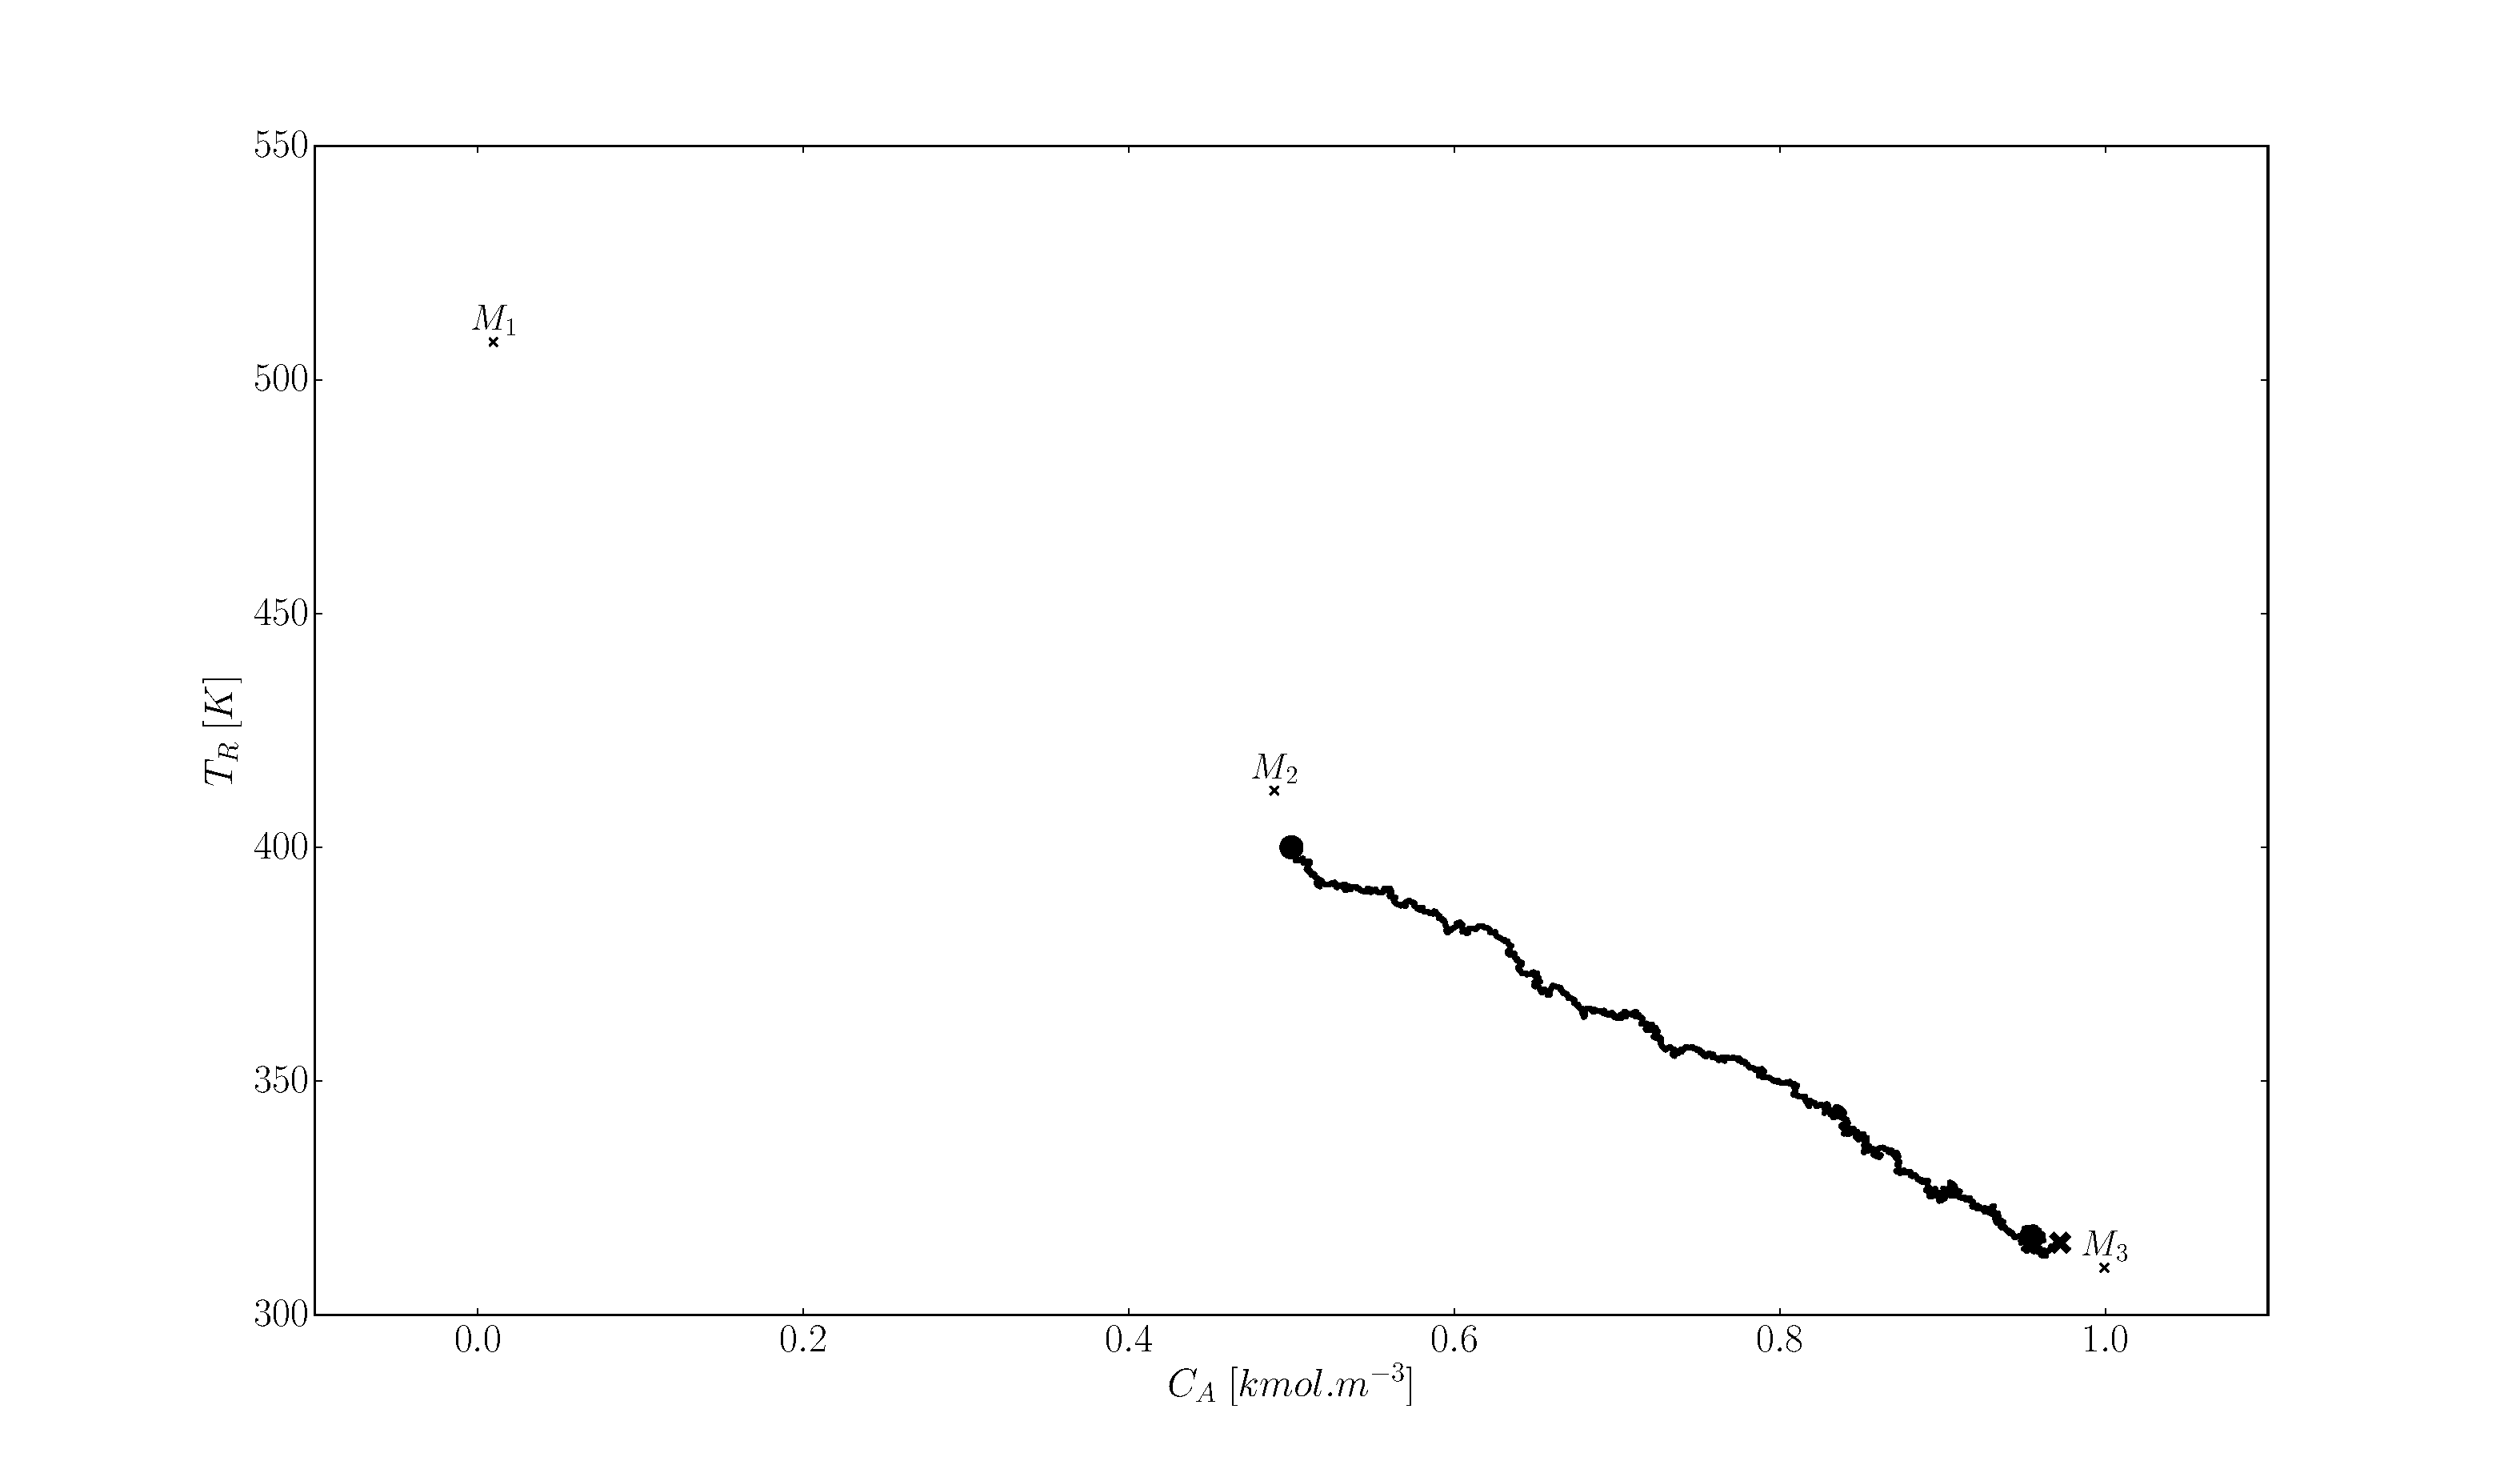
\includegraphics[width=\textwidth]{rbpf_3m_models.pdf}
\caption{State space of the CSTR problem with the position of the 3 linear models superimposed thereupon. The trajectory followed by the system is also shown, the dot is the initial point and the cross the final point.}
\label{fig_3m_models}
\end{figure}
It is clear from Figure \ref{fig_3m_models} that we expect the filter to use $M_2$ initially and then switch to $M_3$ as time progresses. Figure \ref{fig_3m_vage_track} shows how the Rao-Blackwellised particle filter filters the CSTR over a simulation window of 150 minutes. The average concentration error is 22.03\% and the average temperature error is 0.43\% for the state estimator.
\begin{figure}[H] 
\centering
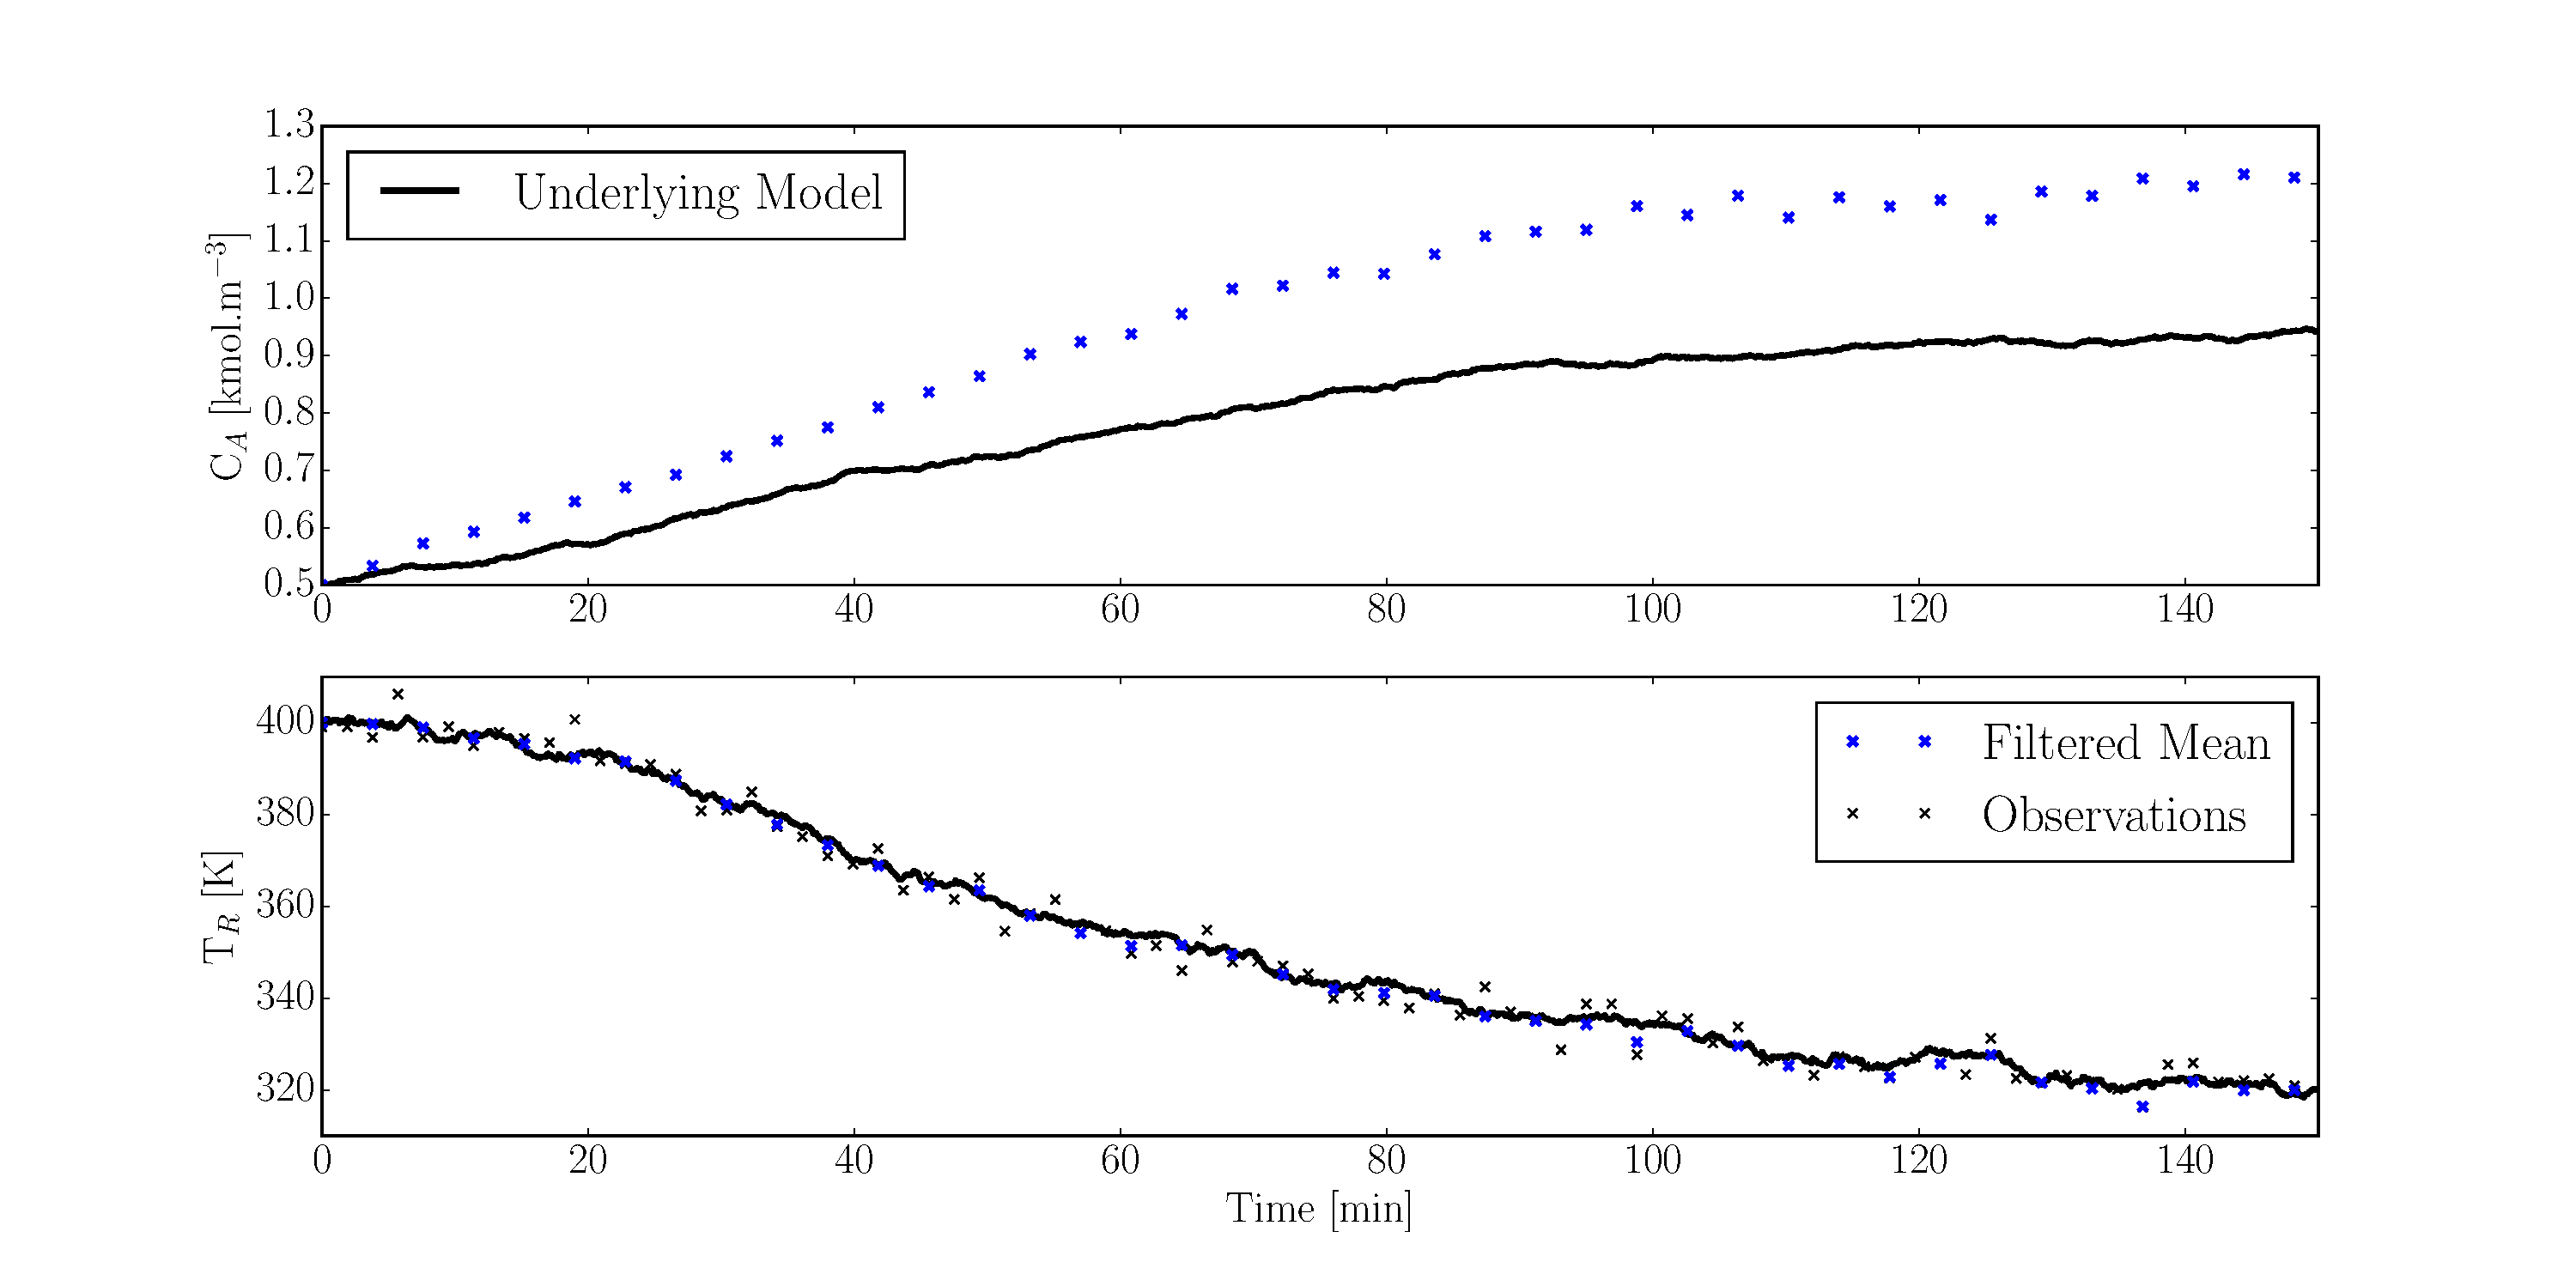
\includegraphics[width=\textwidth]{rbpf_3m_vague_track.pdf}
\caption{Filtering with the Rao-Blackwellised particle filter using 3 linear models and 500 particles. Switch transition matrix $P_1$ was used.}
\label{fig_3m_vage_track}
\end{figure}
Figure \ref{fig_3m_vage_switch} shows the state of the corresponding switching variable $s_t$ over time. Since $s_t$ is a discrete random variable we have that at each time slice $\sum_{i=1}^{M=3} s_t^i = 1$.
\begin{figure}[H] 
\centering
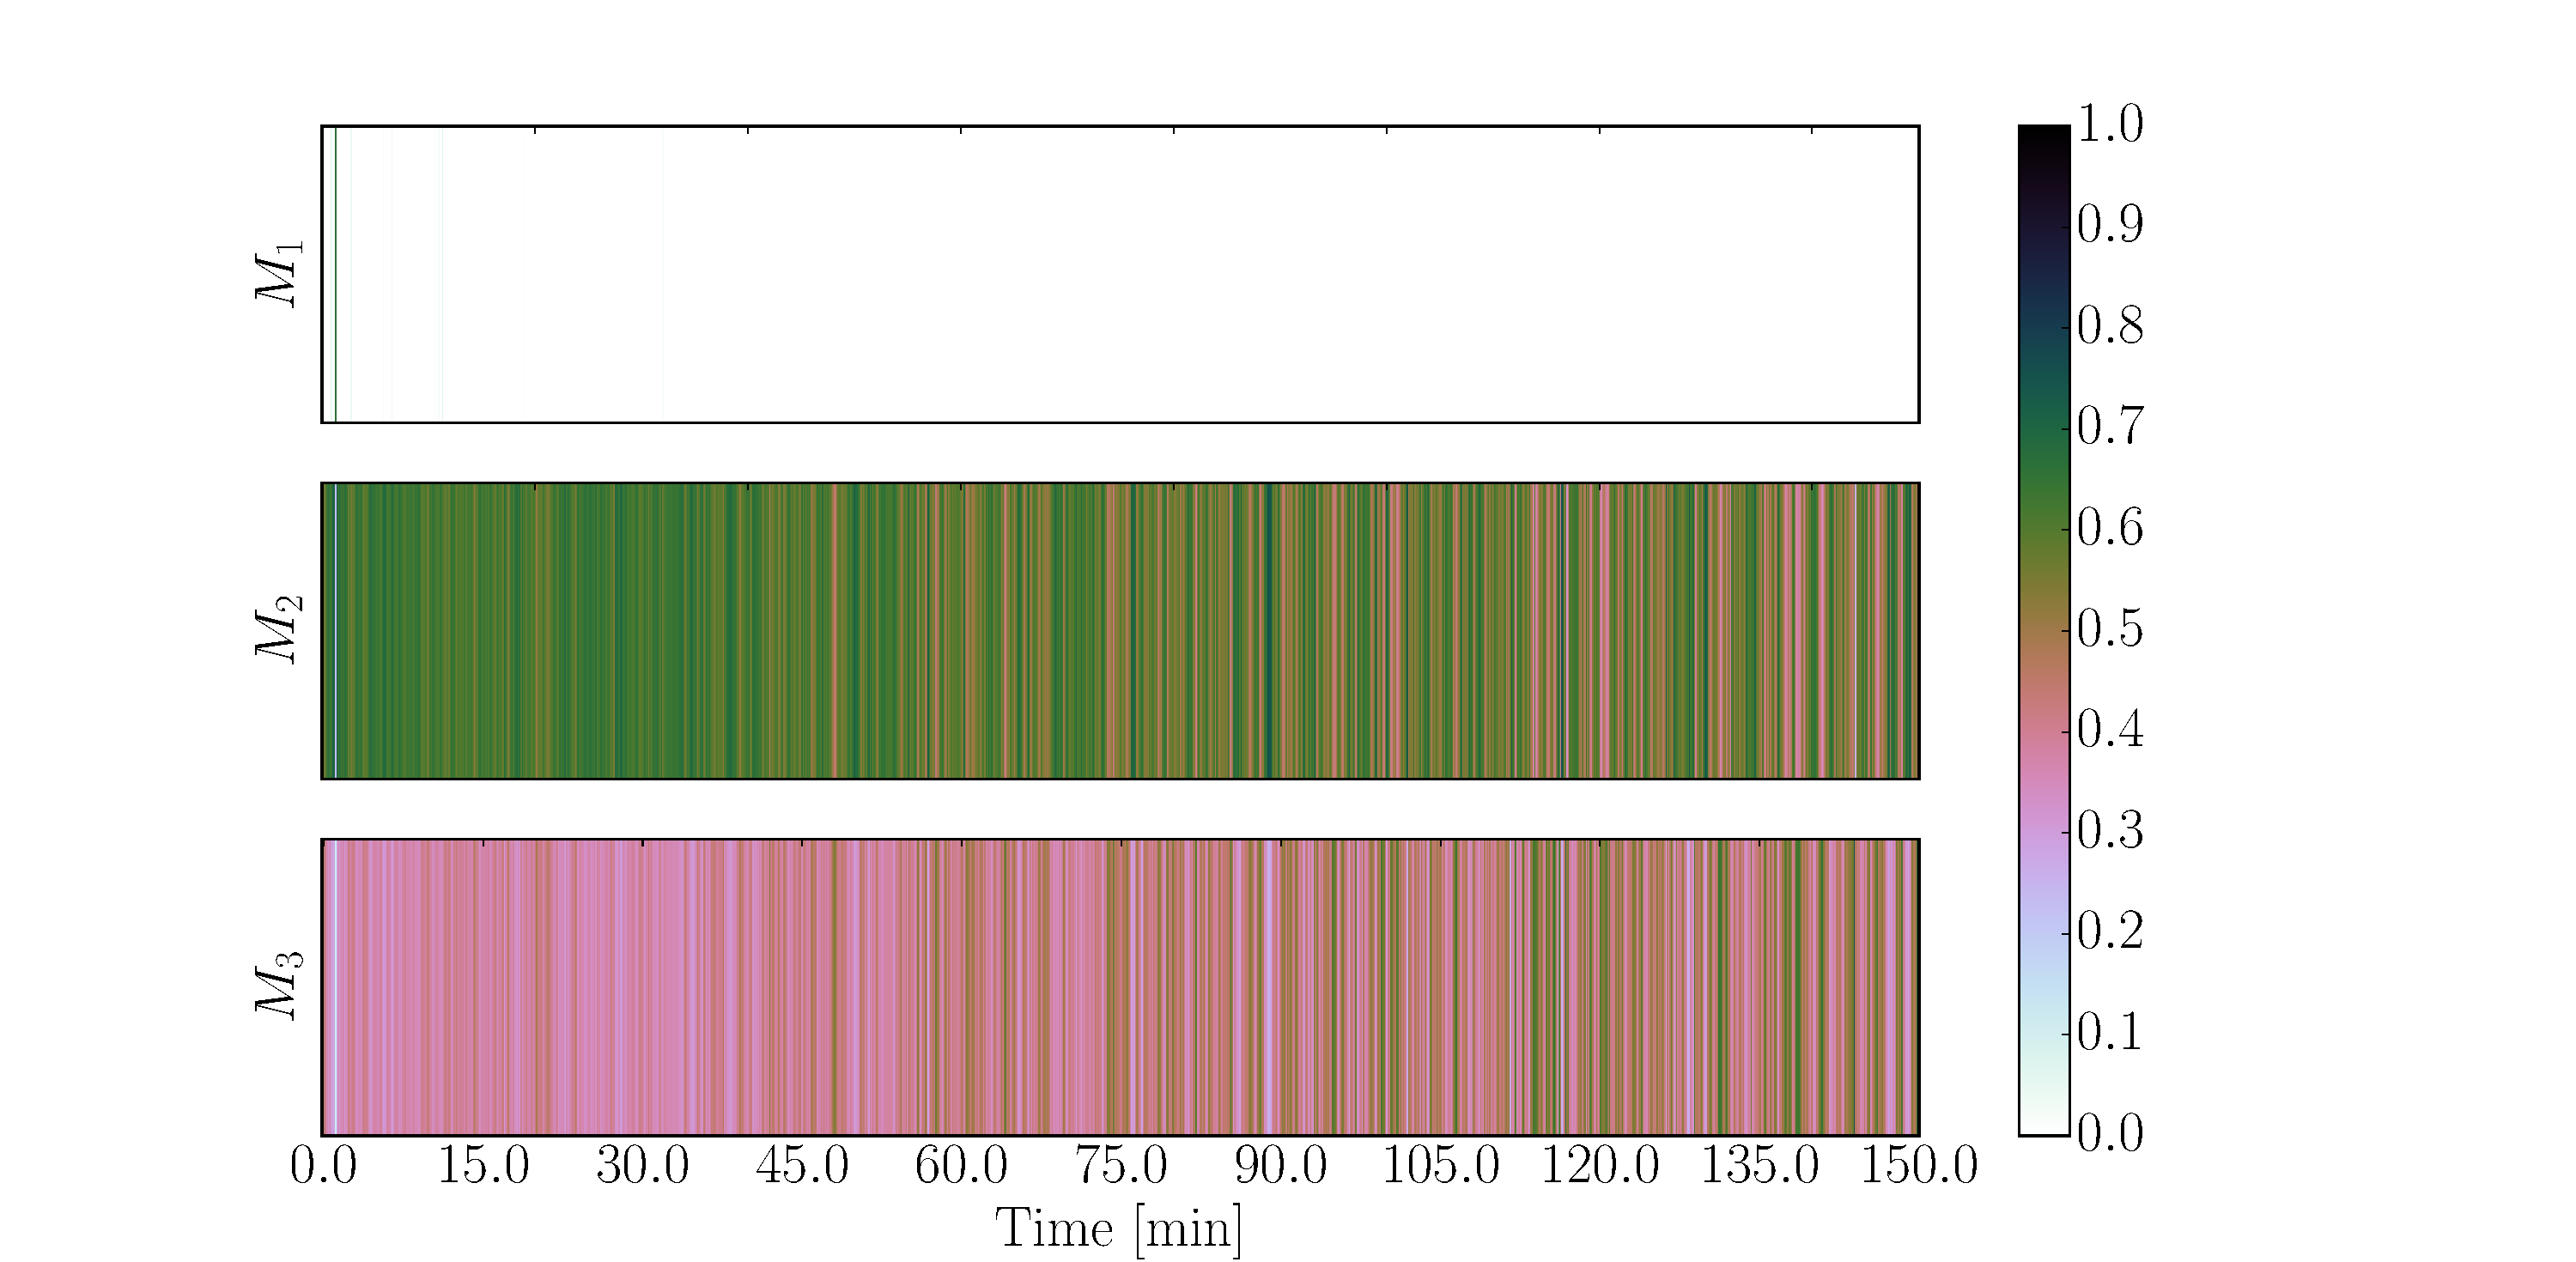
\includegraphics[width=\textwidth]{rbpf_3m_vague_switch.pdf}
\caption{State of the switching variable $s_t$ over time. The weight indicates the sum of the particle weights per model.}
\label{fig_3m_vage_switch}
\end{figure}
From Figure \ref{fig_3m_vage_track} we see that the filtering error is quite large in the unmeasured state. This has been the trend when performing inference on an unmeasured state, however the magnitude of the error does not justify the use of the more complicated graphical model. Additionally, we see that there is no clear switching point in Figure \ref{fig_3m_vage_switch} - the filter relies on both $M_2$ an $M_3$ to estimate the state throughout the simulation. This is contrary to what we expected based on Figure \ref{fig_3m_models}.

Figure \ref{fig_3m_track} shows how the Rao-Blackwellised particle filter filters the CSTR over a simulation window of 150 minutes using $P_2$. The average concentration error is 4.56\% and the average temperature error is 0.23\% for the state estimator. This is a vast improvement over the case where $P_1$ was used.
\begin{figure}[H] 
\centering
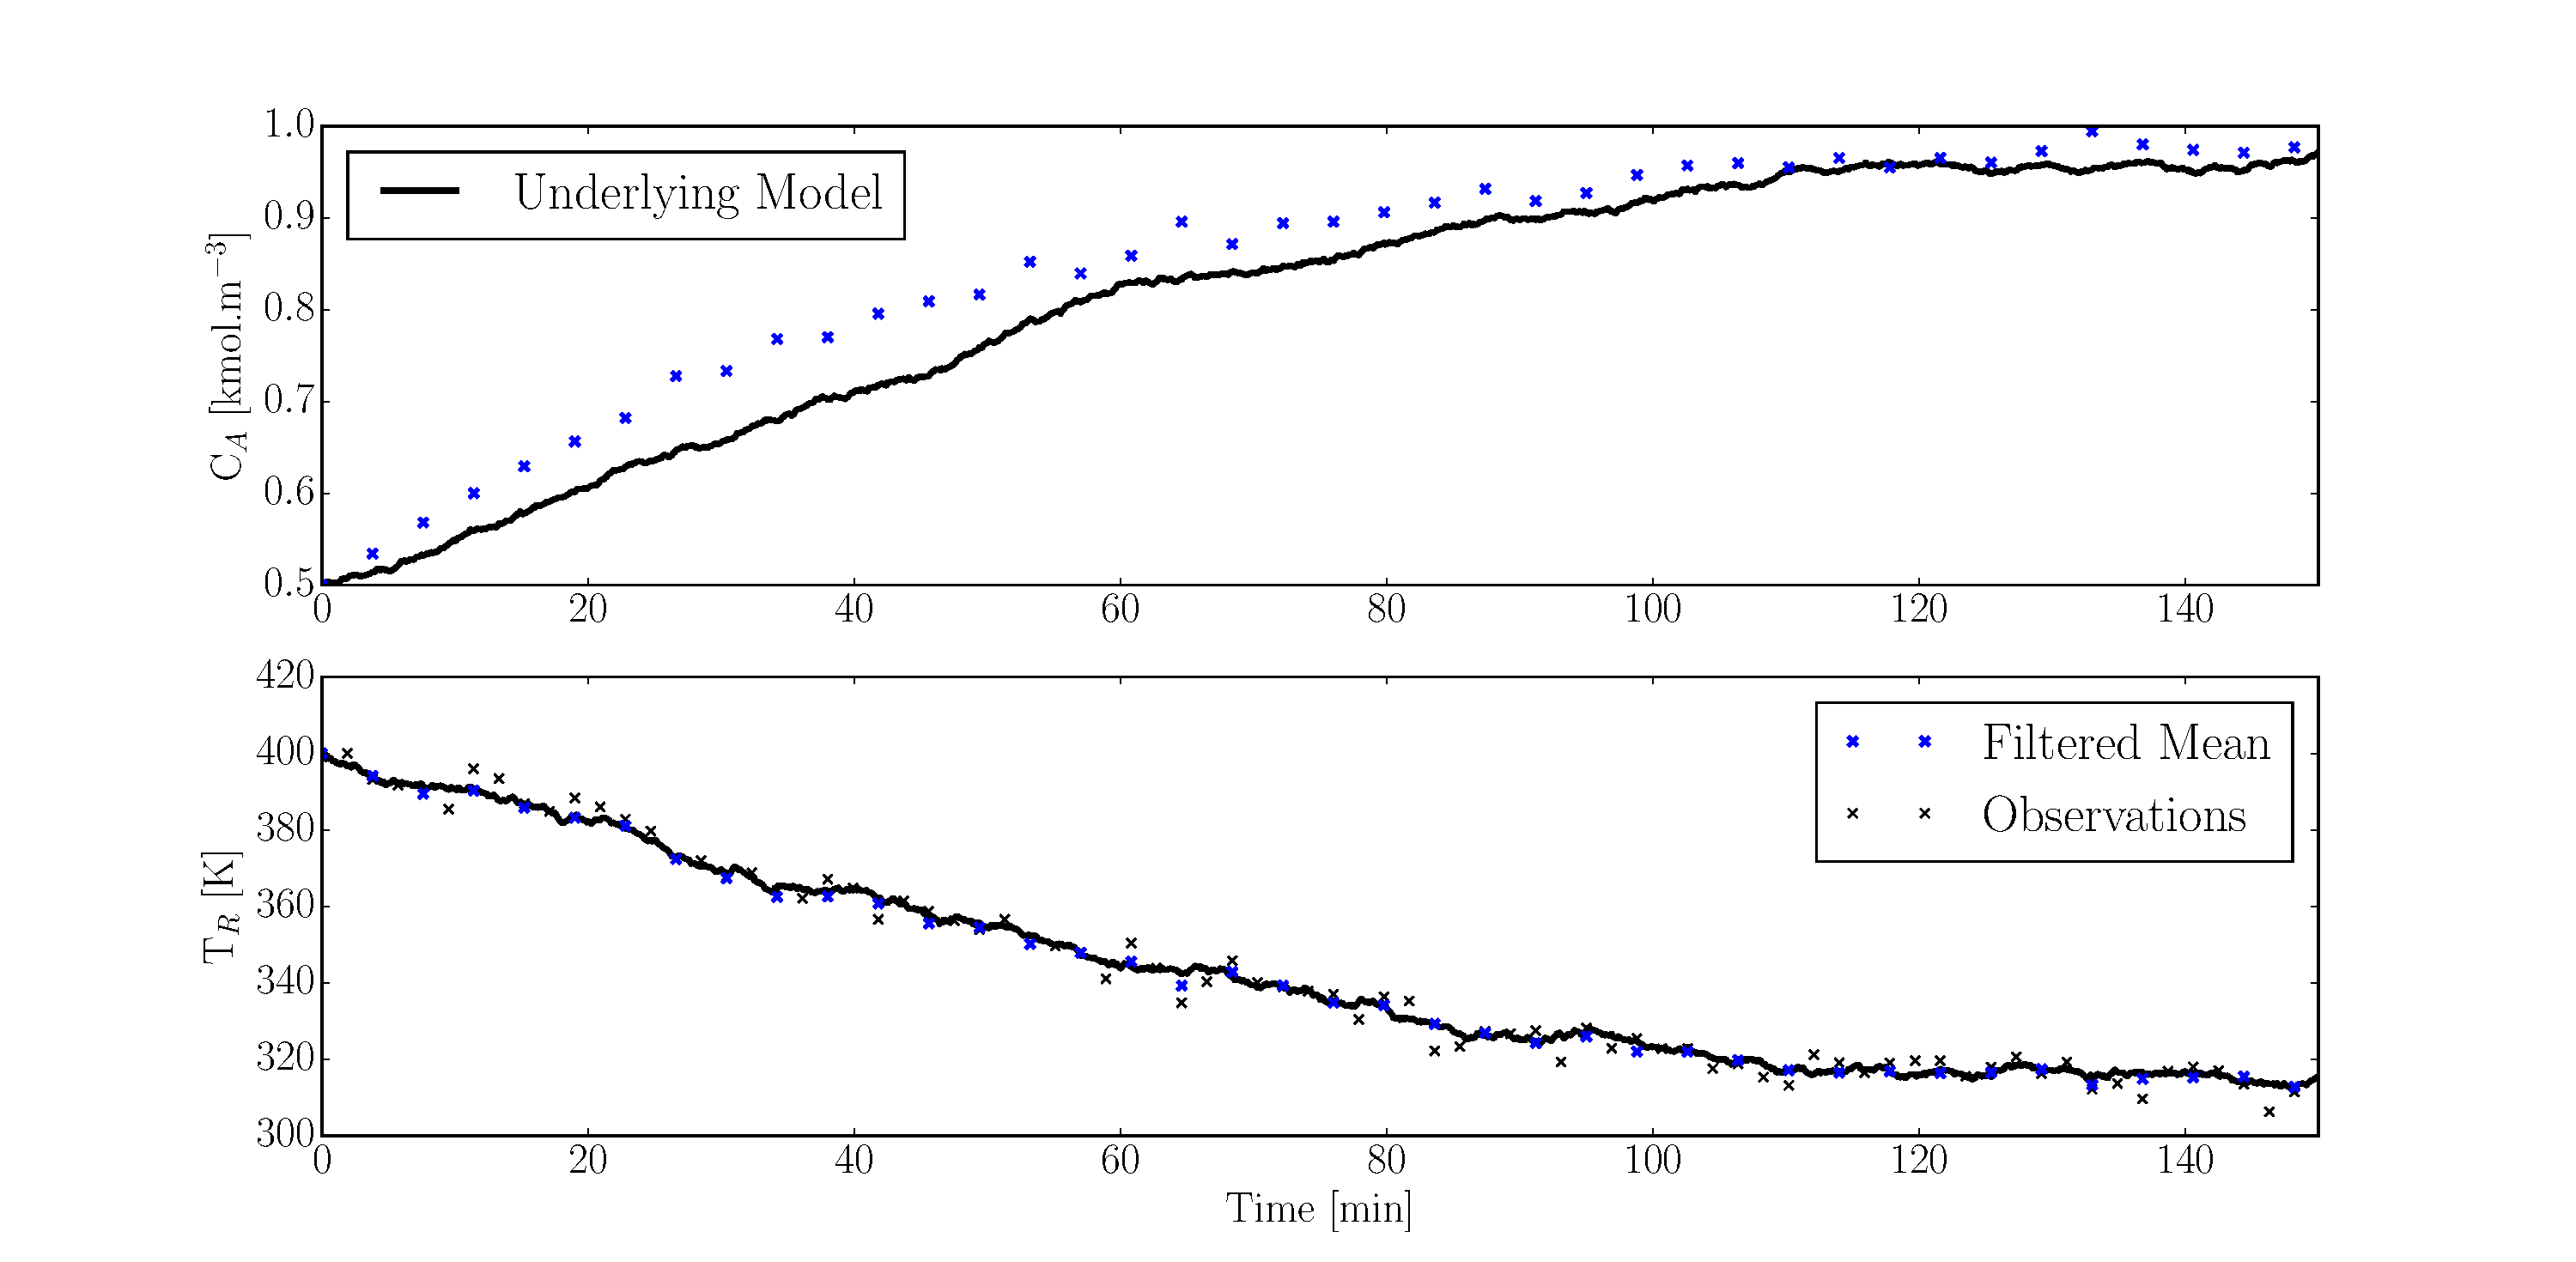
\includegraphics[width=\textwidth]{rbpf_3m_track.pdf}
\caption{Filtering with the Rao-Blackwellised particle filter using 3 linear models and 500 particles. Switch transition matrix $P_2$ was used.}
\label{fig_3m_track}
\end{figure}
Figure \ref{fig_3m_switch} shows the state of the corresponding switching variable $s_t$ over time.
\begin{figure}[H] 
\centering
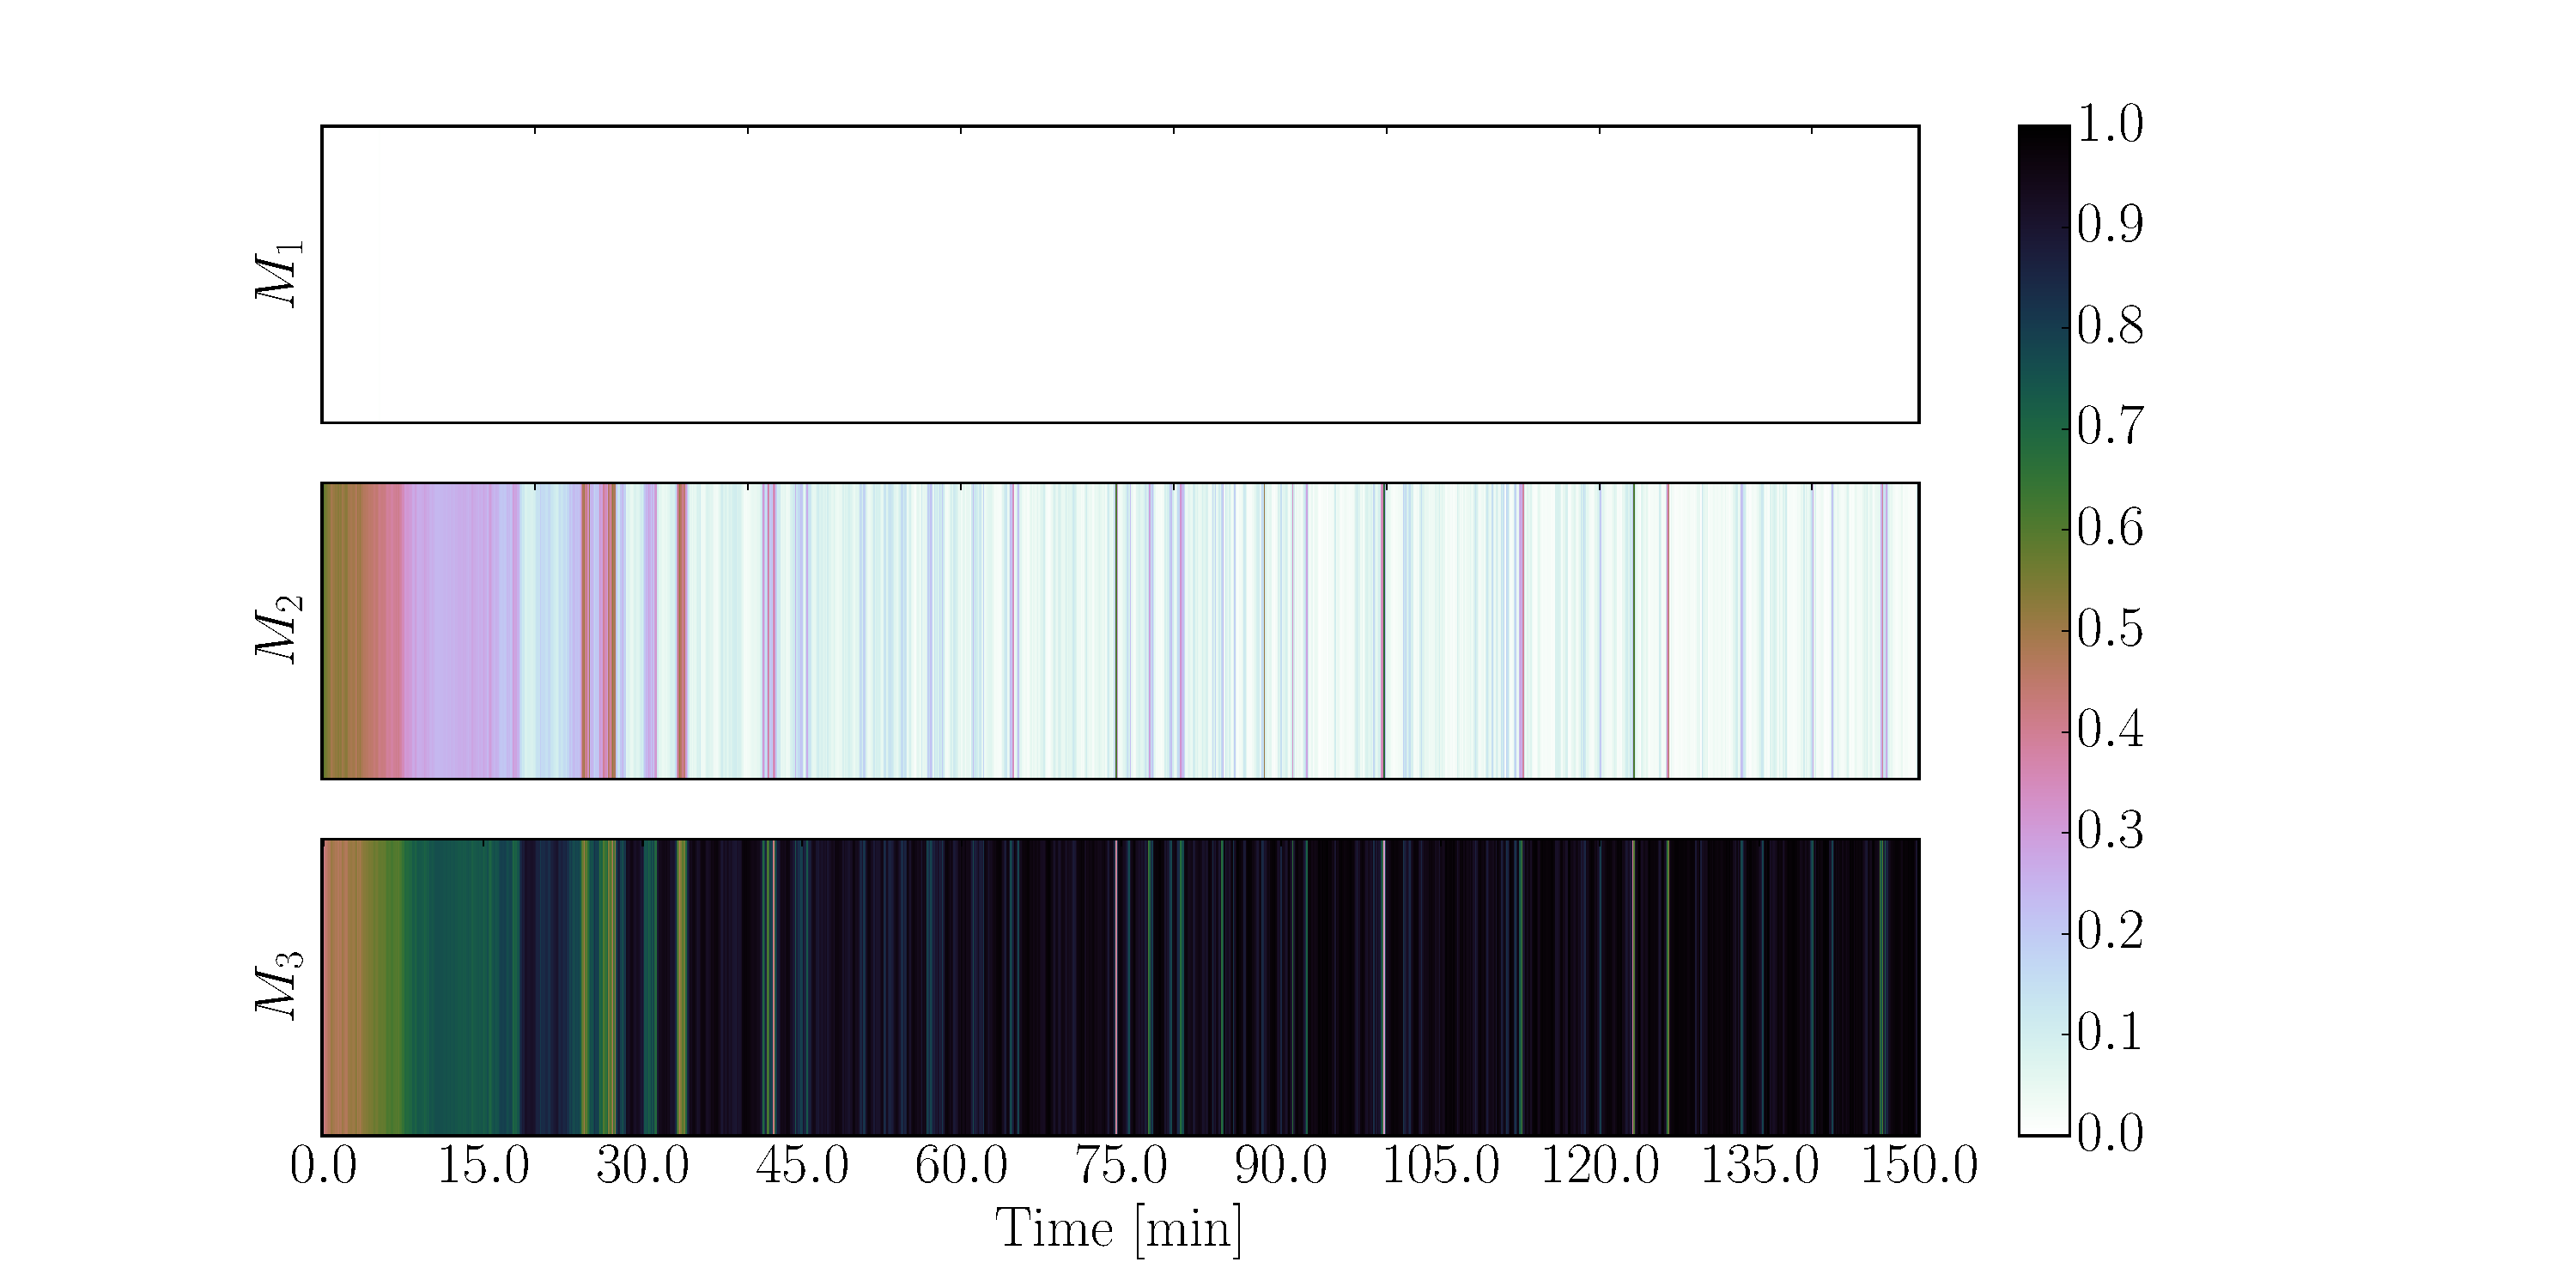
\includegraphics[width=\textwidth]{rbpf_3m_switch.pdf}
\caption{State of the switching variable $s_t$ over time. The weight indicates the sum of the particle weights per model.}
\label{fig_3m_switch}
\end{figure}
Unlike Figure \ref{fig_3m_vage_switch} we do see a clear model transition around the 20 minute mark in Figure \ref{fig_3m_switch}. This is the behaviour we expected - as the system moves away from the unstable operating point the corresponding graphical model becomes less important.

These results suggest that the switch transition matrix sets how ``sticky" the model transitions are. The more vague they are, as in the case of $P_1$, the more unsure the filter is about which model is probably generating the observations. On the other hand, in the case of $P_2$, once the filter switched to the higher probability model it stayed there. The reason for this behaviour is simple: in the case of $P_1$ the approximate split of particles per model is equal. Since a relatively large number of particles represent $M_2$ it is reasonable that one of those particle's ``guesses" will be near the observation. The filter then assigns a high weight to the inappropriate model and the cycle continues. In the case of $P_2$, once the model switches the transition matrix ensures that the number of particles representing $M_2$ is greatly reduced. This then improves filtering performance because the unlikely model does not have a large share of the available particles while the more likely model has more.

This behaviour is also desirable because it makes the switching variable have physical significance (not to mention that it improves filtering performance). However, the immediate drawback of the ``sticky" approach is that the filter may be slow to switch models. Additionally if a machine learning approach is not used to infer the values of $P$ it could become a tedious task to set $P$ for a large system. Clearly the values used in $P_2$ were set by hand - more investigation is necessary to determine proper heuristics if this approach should be adopted in practice.

Next we investigate the effect measuring both states has on the accuracy of the filter. Due to the work in Chapters \ref{sec_inf_lin_mods} and \ref{sec_inf_nonlin_mods} we expect that by measuring concentration we will increase the filter accuracy. We use the 3 model filter with $P_2$ to demonstrate that this is the case.

In Figure \ref{fig_3m_track_m2} we see the filtering performance of the Rao-Blackwellised particle filter measuring both states. The average concentration and temperature error is 0.66\% and 0.22\%. This is a significant improvement over the tracking we saw in Figure \ref{fig_3m_track}.
\begin{figure}[H] 
\centering
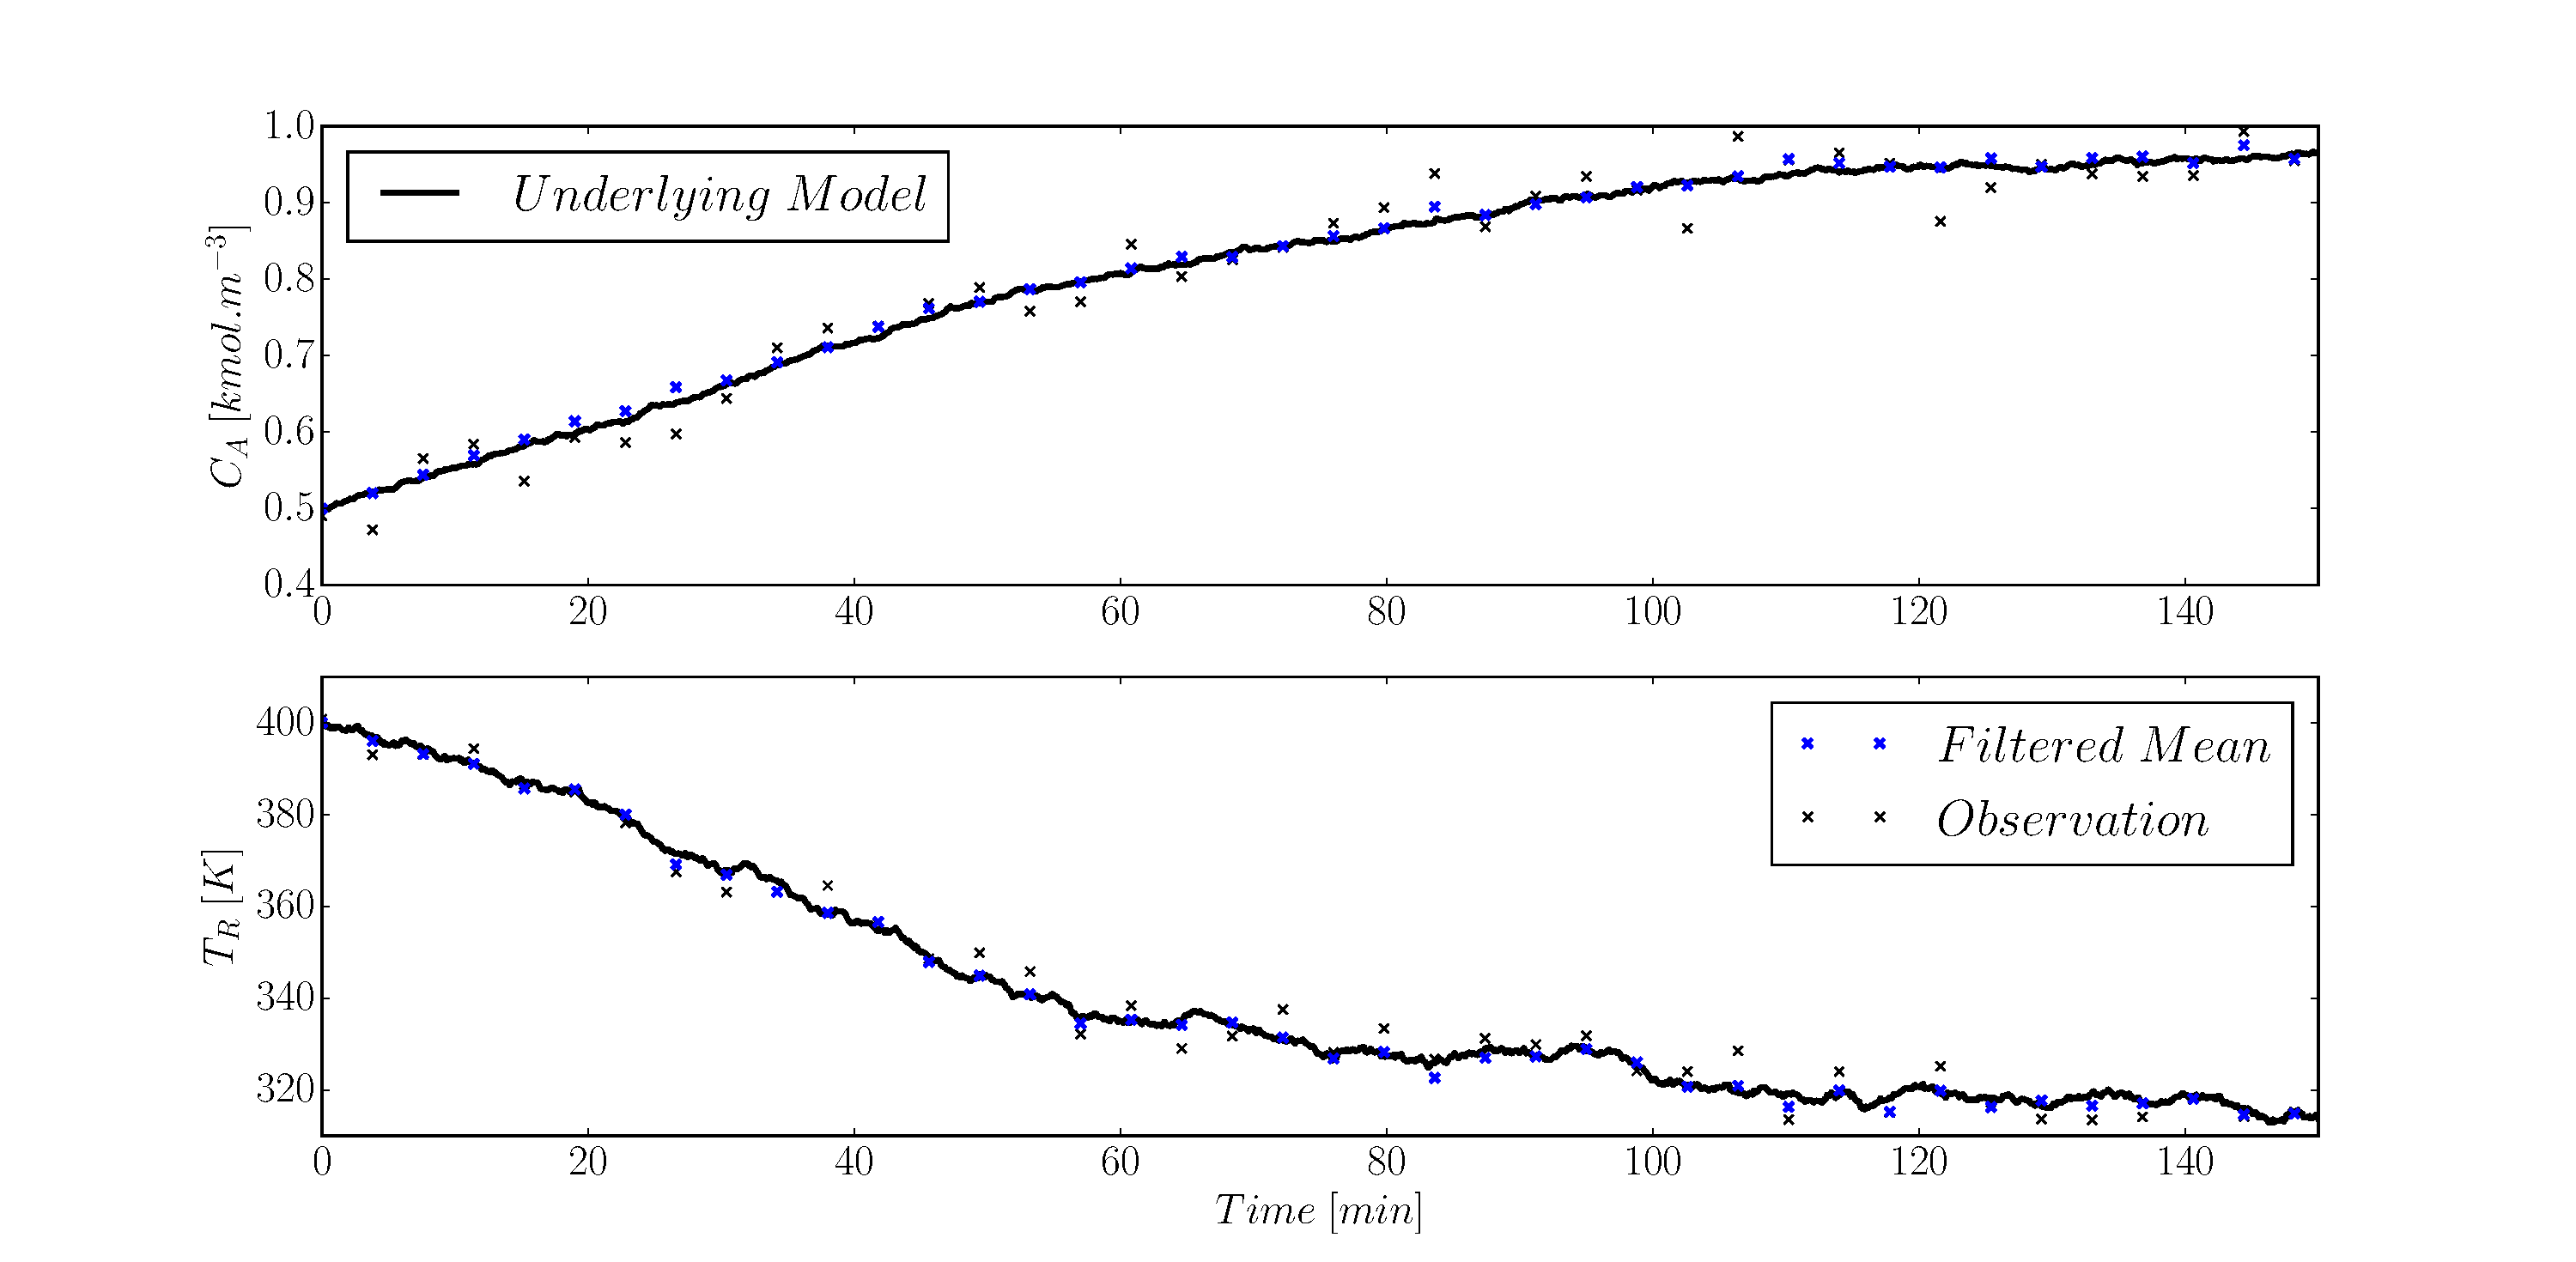
\includegraphics[width=\textwidth]{rbpf_3m_track_m2.pdf}
\caption{Filtering with the Rao-Blackwellised particle filter using 3 linear models and 500 particles. Switch transition matrix $P_2$ was used. Both states are measured.}
\label{fig_3m_track_m2}
\end{figure}
In Figure \ref{fig_3m_switch_m2} we see the state of the switching variable over the simulation run. Like Figure \ref{fig_3m_switch} we also see a clear switch occurring at approximately 15 minutes (actually at 20 minutes when measuring only one state). However, comparing Figures \ref{fig_3m_switch} and \ref{fig_3m_switch_m2} closely we see less ``switching noise" in the latter. The second measurement allows the filter to compare both state predictions to discern between models. This is clearly beneficial.
\begin{figure}[H] 
\centering
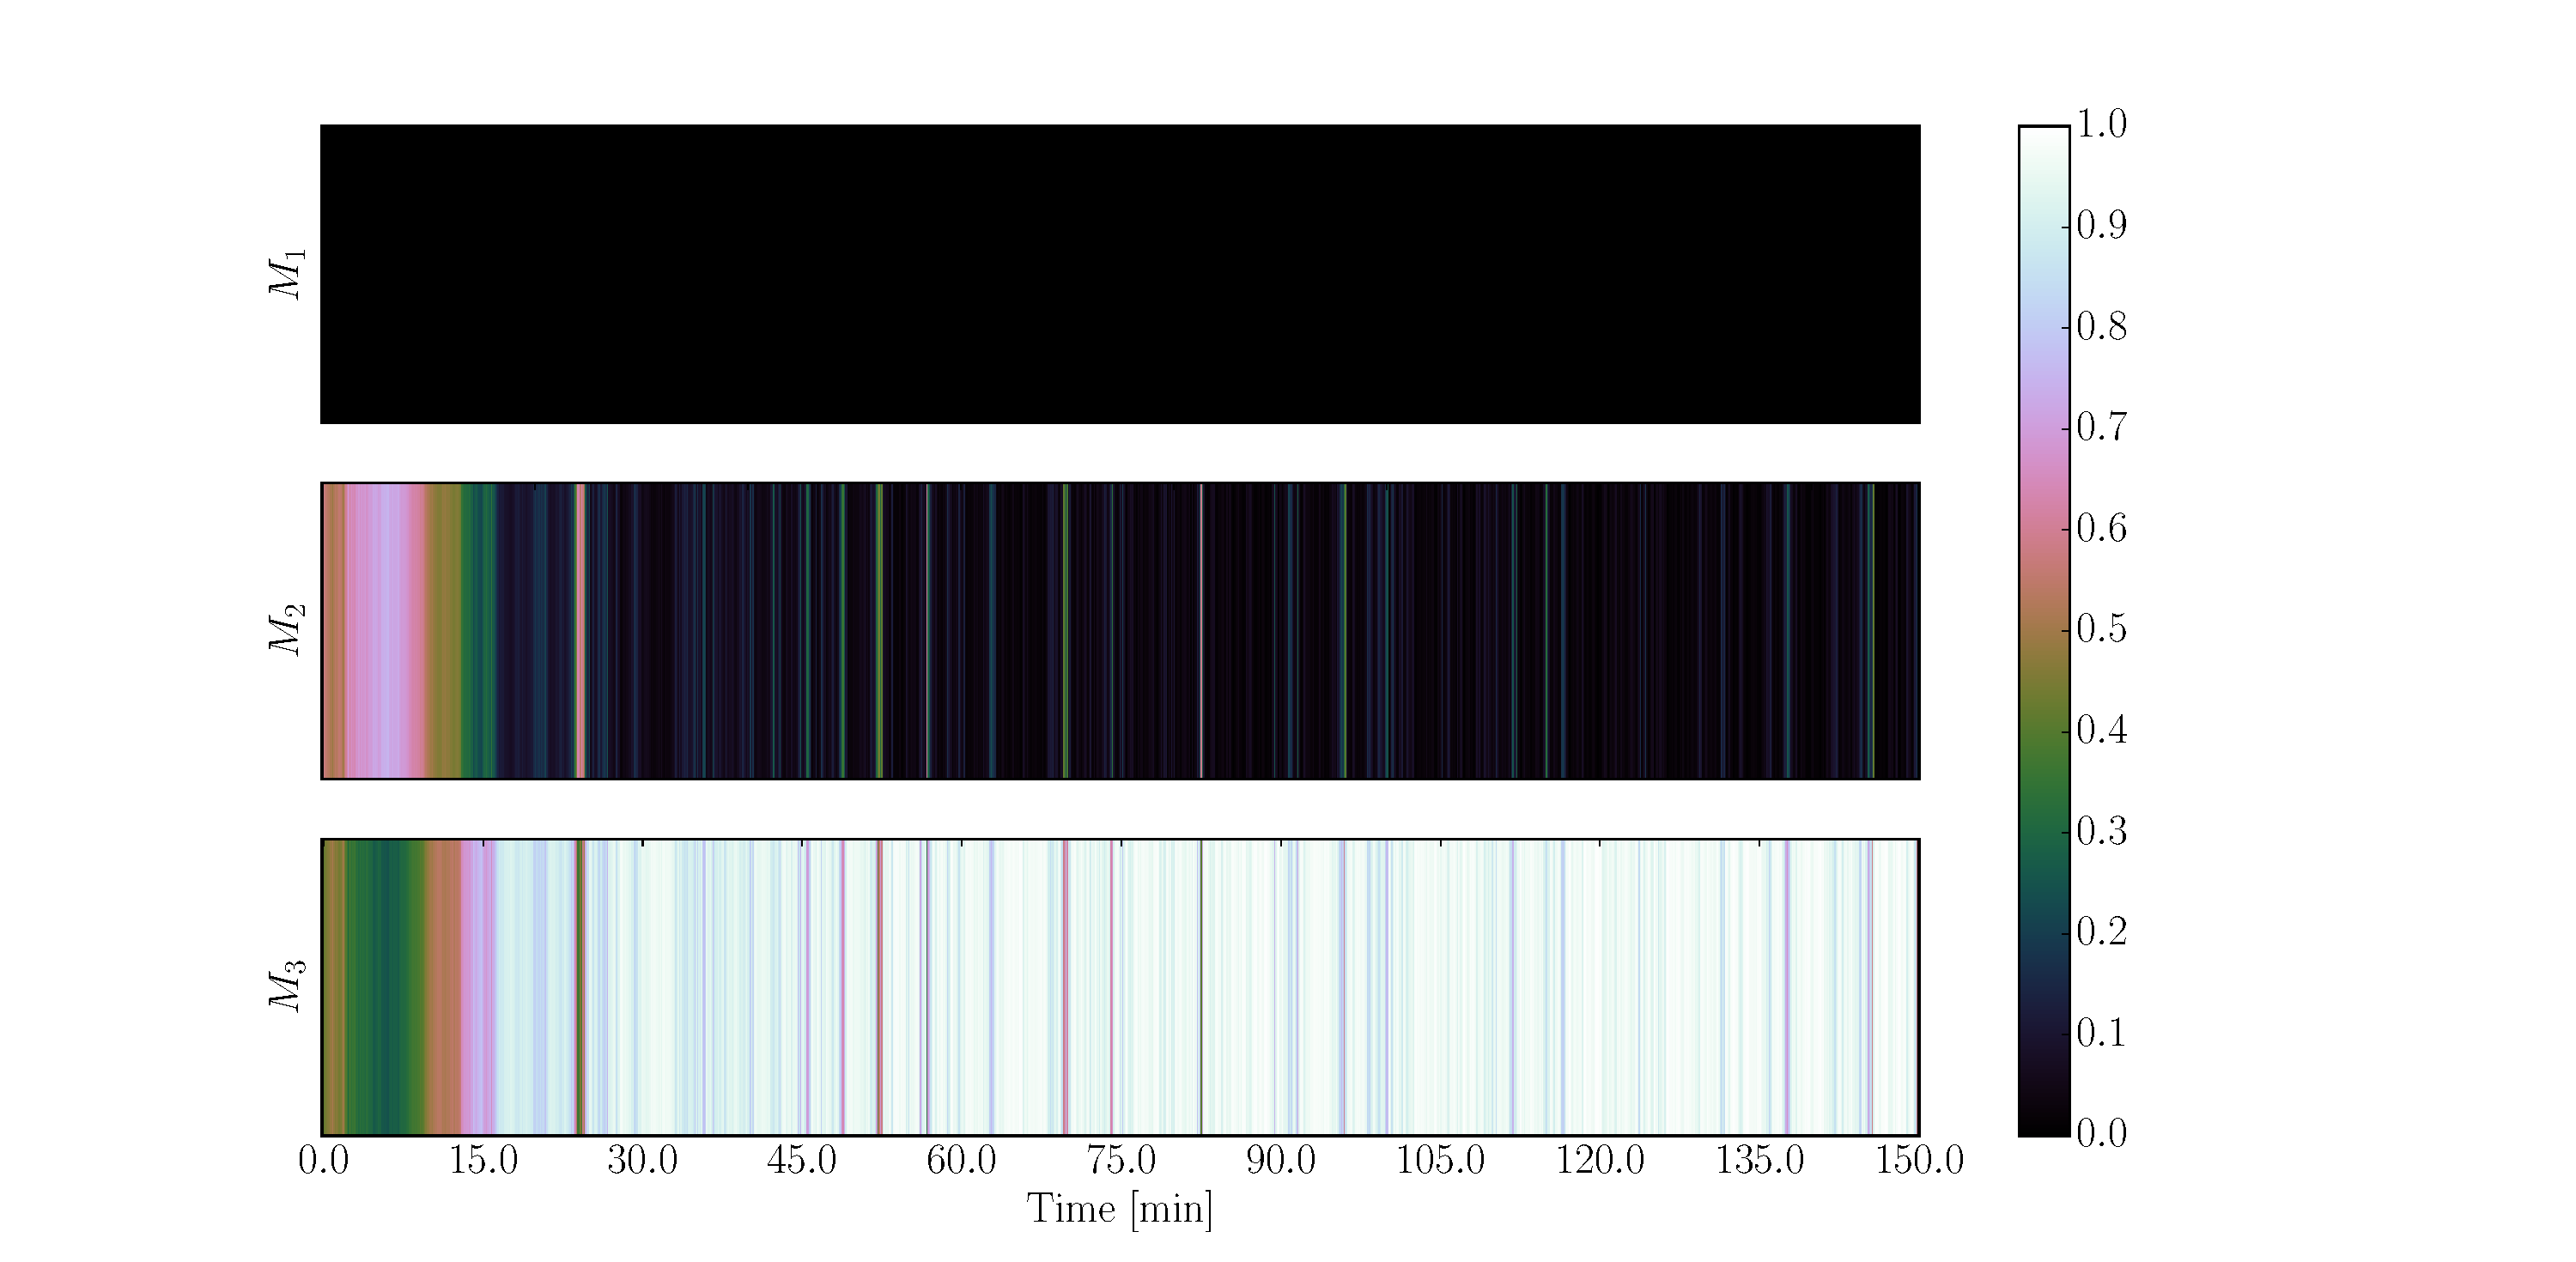
\includegraphics[width=\textwidth]{rbpf_3m_switch_m2.pdf}
\caption{State of the switching variable $s_t$ over time. The weight indicates the sum of the particle weights per model.}
\label{fig_3m_switch_m2}
\end{figure}
Finally, we investigate the effect using more models has on the filter which measures both states. We use the same 3 model filter as before (using $P_2$) but compare it to a 7 model filter. The state transition matrix for the 7 model filter is shown in (\ref{eq_state_trans7}). We again assume that the state and measurement noise is common to all models and that they all share the same observation matrix $C$.
\begin{equation}
P_3 = \begin{pmatrix}
0.98 & 0.00 & 0.00 & 0.00 & 0.00 & 0.01 & 0.00 \\
0.00 & 0.98 & 0.00 & 0.01 & 0.01 & 0.01 & 0.00 \\
0.01 & 0.00 & 0.98 & 0.00 & 0.00 & 0.01 & 0.01 \\
0.00 & 0.00 & 0.00 & 0.98 & 0.00 & 0.01 & 0.00 \\
0.00 & 0.01 & 0.00 & 0.00 & 0.99 & 0.00 & 0.00 \\
0.01 & 0.01 & 0.01 & 0.01 & 0.00 & 0.96 & 0.00 \\
0.00 & 0.00 & 0.01 & 0.00 & 0.00 & 0.00 & 0.99 \\
\end{pmatrix}
\label{eq_state_trans7}
\end{equation}
The values of $P_3$ were set using the same reasoning as before. Figure \ref{fig_7m_models} show state trajectory of the system (like Figure \ref{fig_3m_models}) but with the additional models superimposed thereupon. Clearly $M_5$, $M_6$ and $M_7$ correspond to high temperature, unstable and low temperature operating points. 
\begin{figure}[H] 
\centering
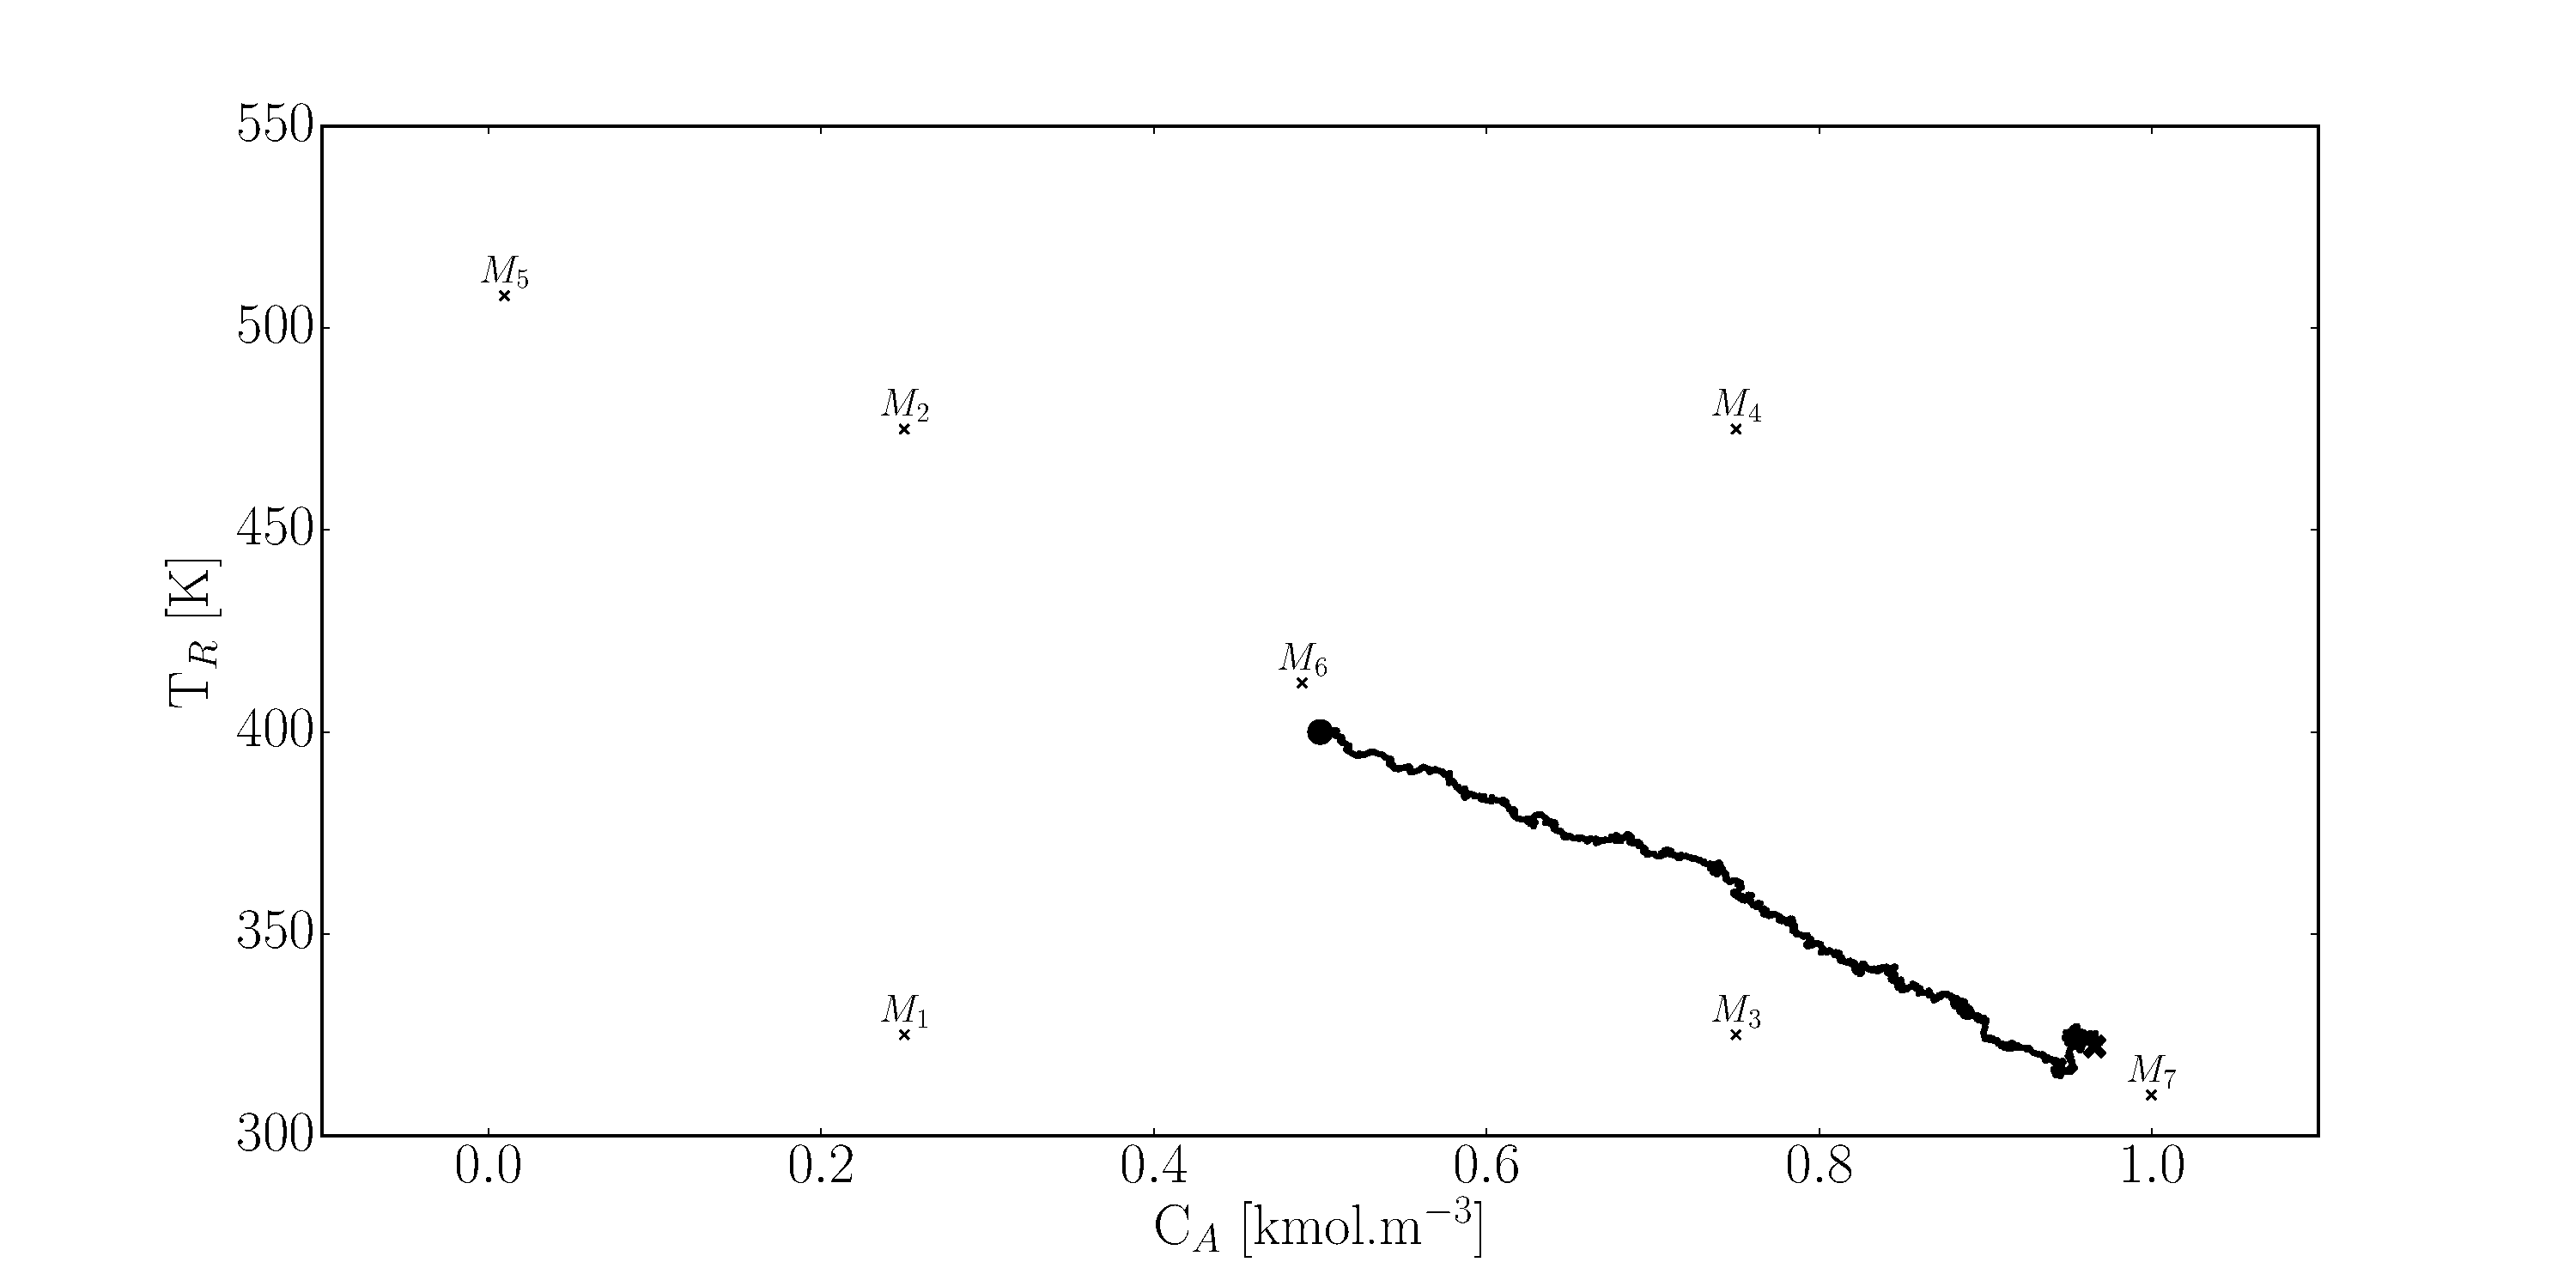
\includegraphics[width=\textwidth]{rbpf_7m_models.pdf}
\caption{State space of the CSTR problem with the position of the 7 linear models superimposed thereupon. The trajectory followed by the system is also shown, the dot is the initial point and the cross the final point.}
\label{fig_7m_models}
\end{figure}
Figure \ref{fig_7m_track} shows the effectiveness of the filter over the simulation window. The average concentration and temperature error is 0.71\% and 0.23\% respectively. 
\begin{figure}[H] 
\centering
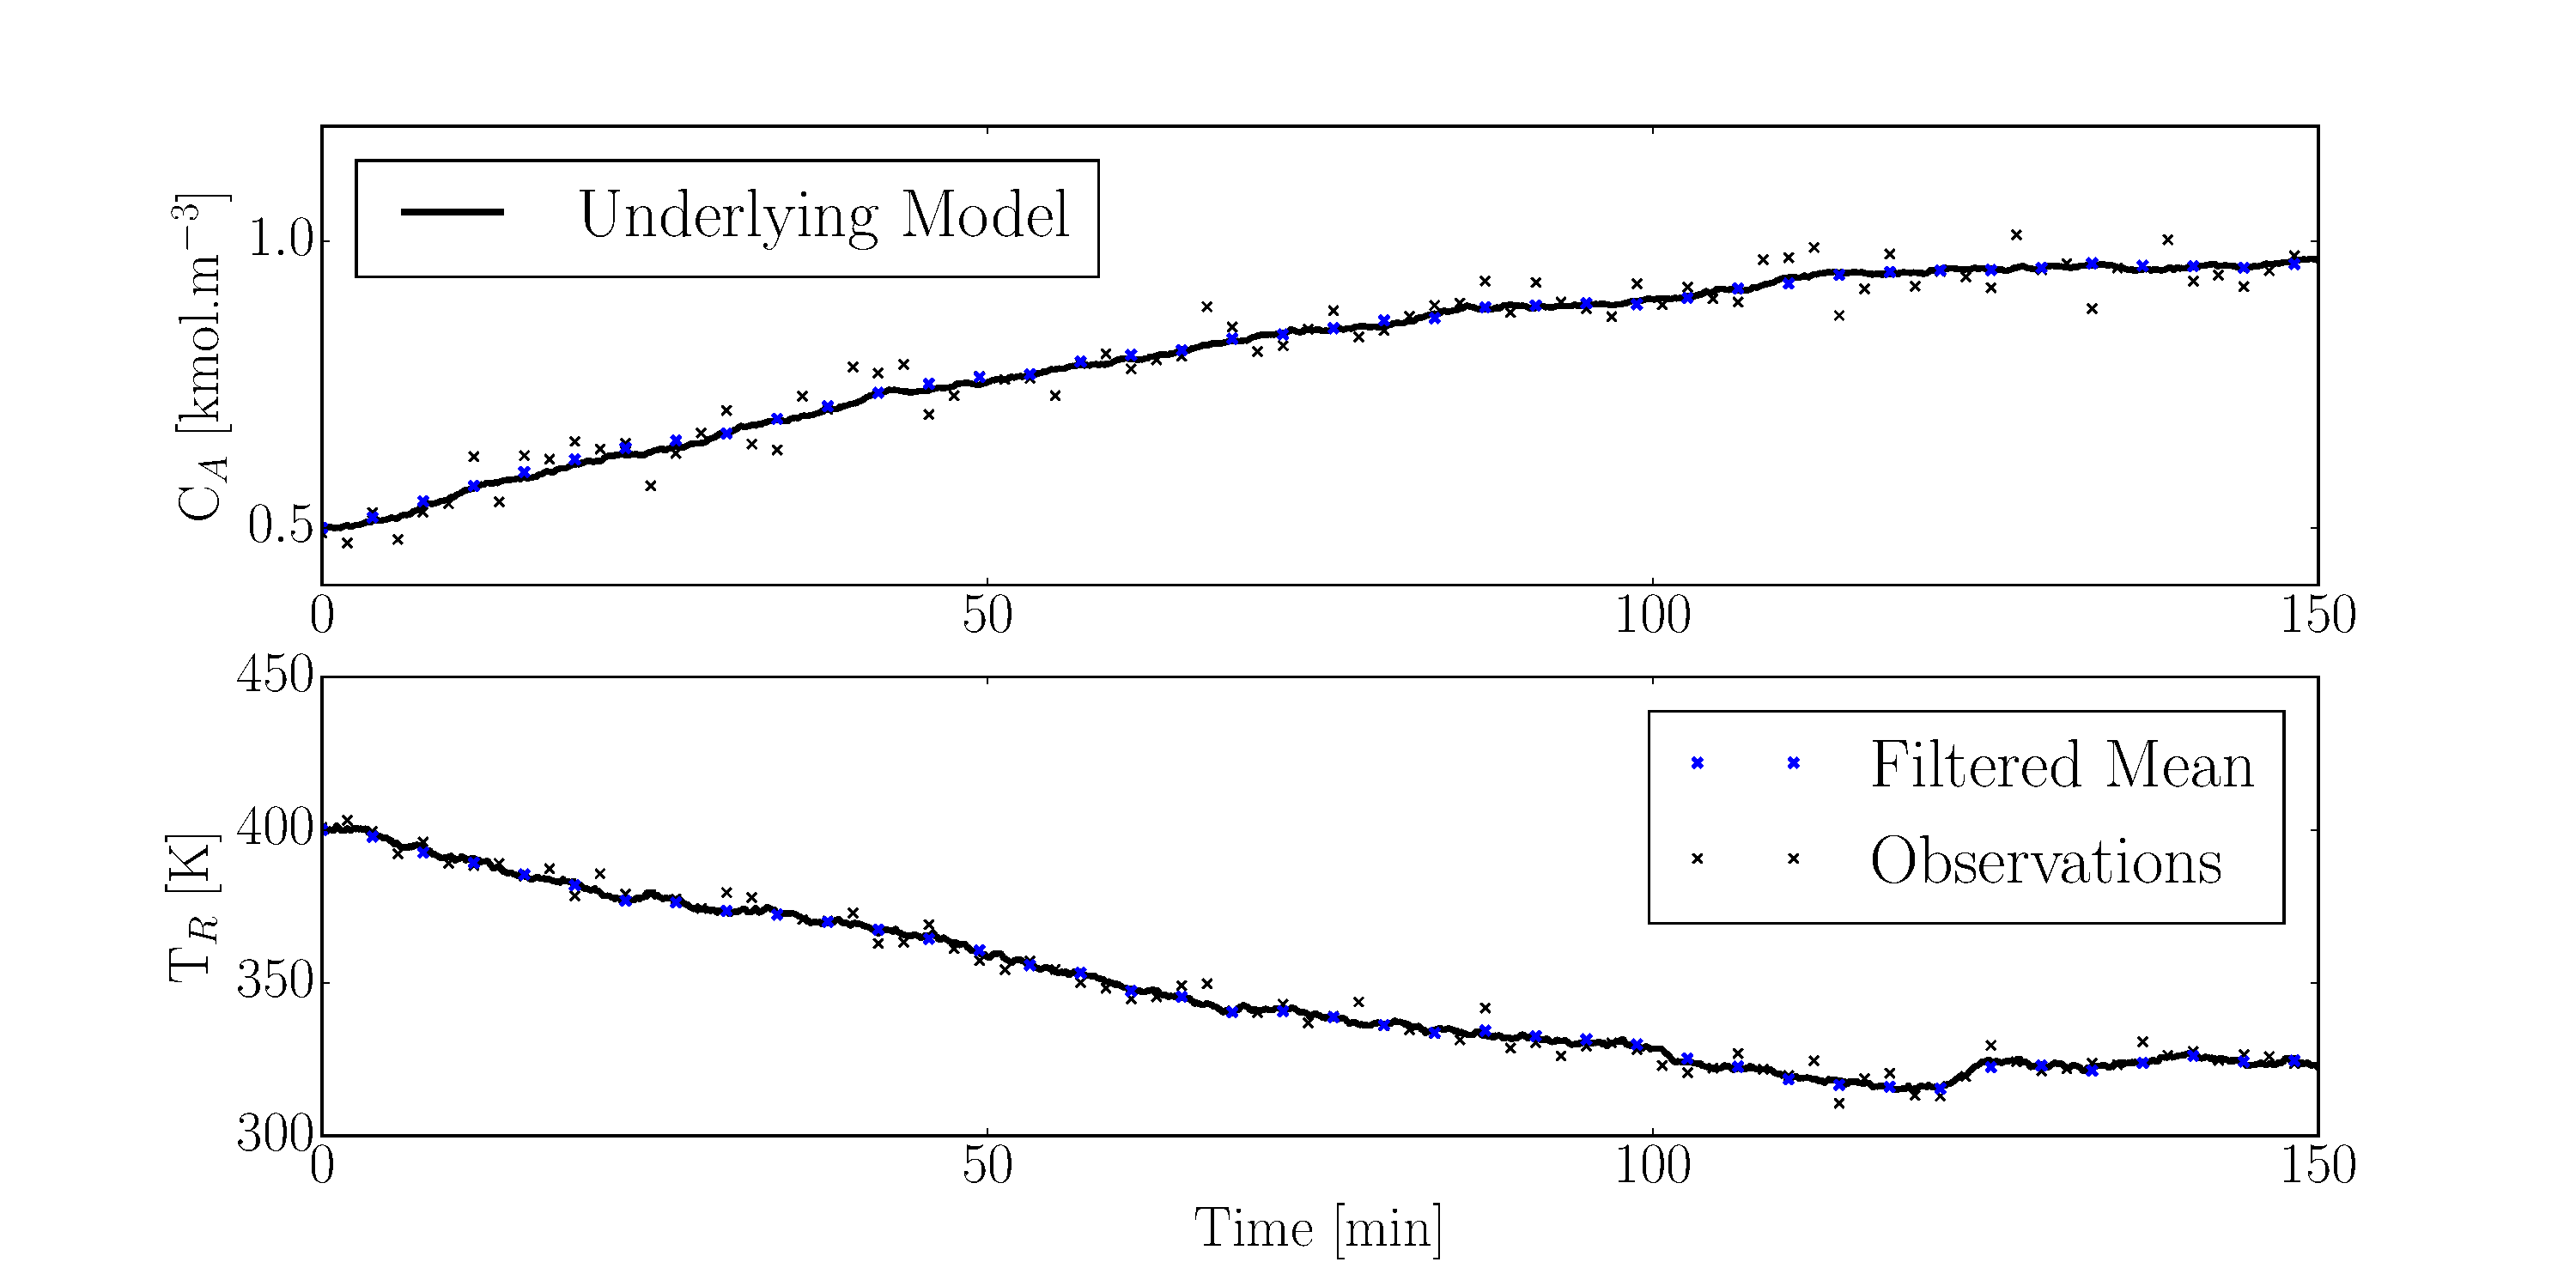
\includegraphics[width=\textwidth]{rbpf_7m_track.pdf}
\caption{Filtering with the Rao-Blackwellised particle filter using 7 linear models and 500 particles. Switch transition matrix $P_3$ was used.}
\label{fig_7m_track}
\end{figure}
Interestingly enough we actually observe worse tracking performance when more models are used compared to the 3 model case with $P_2$. We expected the additional models to increase the effectiveness of the filter. Figure \ref{fig_7m_switch} shows the state of the corresponding switching variable $s_t$ over time. A possible explanation for the performance degradation is evident here.
\begin{figure}[H] 
\centering
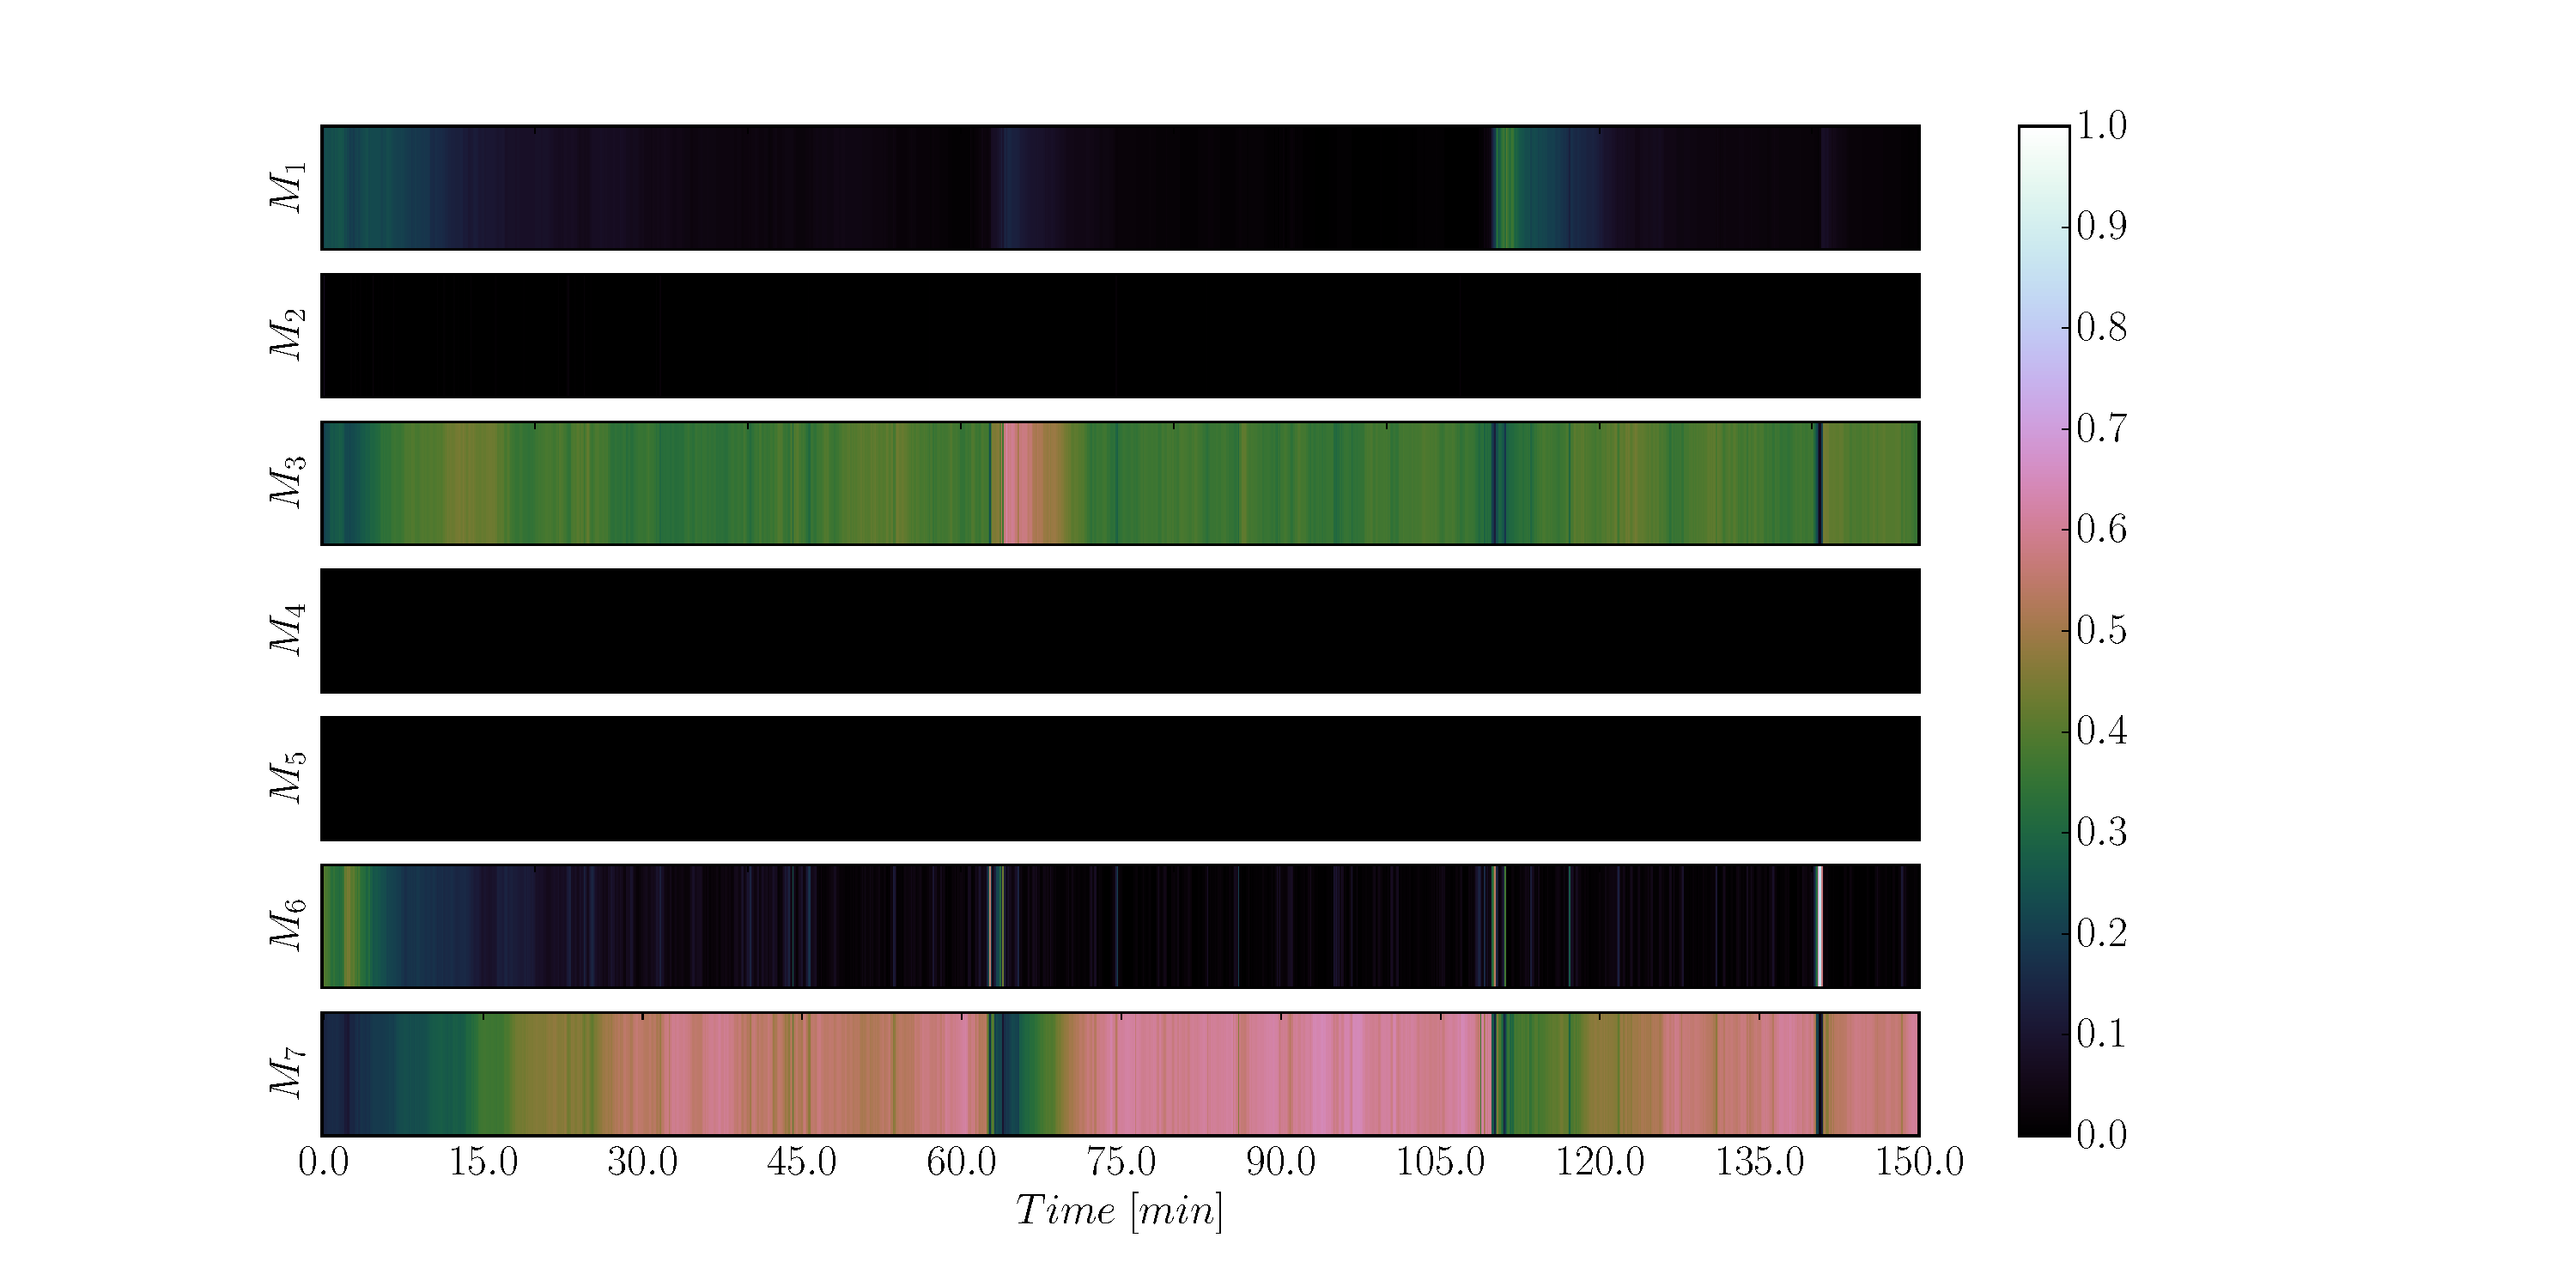
\includegraphics[width=\textwidth]{rbpf_7m_switch.pdf}
\caption{State of the switching variable $s_t$ over time. The weight indicates the sum of the particle weights per model.}
\label{fig_7m_switch}
\end{figure}
We certainly expected $M_7$ to be the dominant model near the end of the simulation; however $M_3$, while close to the low temperature operating point, played a significant role in the state estimate throughout the simulation. The filter uses a weighted combination of model predictions to estimate the current state; it is evident that there were a non-negligible number of particles which maintained the $M_3$ hypothesis. This implies that less particles were available to use the $M_7$ model and thus we see worse performance.

The crux of the problem is model overlap. While it is clear to a human that the system should only use $M_7$ near the end of the simulation the algorithm has no way of knowing this. It infers this based on the predictive ability of the models. Clearly $M_7$, $M_3$ and to a lesser extent $M_1$ and $M_6$ were all able to accurately predict the current state. For this reason they have non-negligible weights in Figure \ref{fig_7m_switch}.  

We have in fact already come across this problem in Figures \ref{fig_3m_vage_track} and \ref{fig_3m_vage_switch}. We saw that it is possible to attenuate this problem by making the switching transition matrix ``stickier". Unfortunately this does not solve the underlying problem - the models are not different enough. Using more models would only make this problem worse.

It should be added that this problem is not necessarily bad for inference. The model switching and weighting allows the filter to accurately track regions between the linear models i.e. regions where no one model is accurate. From a filtering perspective this can be beneficial.

In the next chapter we implement switching model predictive controllers using the Rao-Blackwellised particle filter to select the best model for prediction.